% 
% 文書の構成
% 序論    [1]問う       目的(introduction)      自分の研究で明らかにしたい問いを示します.
%         [2]調べる     先行研究(introduction)  関連する先行研究を紹介し,本研究のオリジナリティを示します.
%         [3]選ぶ       資料と方法(Material and Method)  問いを明らかに検証するためのデータの概要と方法を示します.
% 本論    [4]確かめる   結果と分析(Results)     分析を経た調査の結果を示し,問いに答えます.    
%         [5]裏付ける   考察(Discussion)        なぜそのような結果になるのか,その理由を考えます.
% 結論    [6]まとめる   結論(Conclusion)         [1]〜[5]の論証のプロセスを要約し,今後の課題を示します.
%
% IMRAD, イントロ,方法,結果,議論,理系の学術論文
% 方法:物理学的基礎知識,Processing
% 開発結果
% ソフトの振る舞い,ソフト試行錯誤の過程
% 

% outputの時の判断基準
% 先行研究,資料と方法:あるもんしらべた
% 結果と分析:ないもんをつくった
%
% ruby_noviceの簡単な使用法を書く
% 開発したソフトの振る舞い(使用法)を記述することによって,
% どのようなソフトかを読む人が理解できるように
% だから,何が必要かというのを
% divide and quanquar:各個撃破
% プレゼンの極意:むずいとこはあっさりと,易しいとこをこってりと

%スタイル,パッケージの設定
\documentclass[12pt,a4]{jreport}%chapterが使えるスタイル
\usepackage[dvipdfmx]{graphicx}%図の挿入のためのパッケージ
\usepackage{amsmath}
\usepackage{setspace}
\usepackage{amssymb}
\usepackage{ascmac}
\usepackage{framed}
\usepackage{url}
\usepackage{subcaption}

%\usepackage{wrapfig}	
%\usepackage[dvipdfmx]{graphicx}
%\usepackage{url}
%\usepackage{here}
%\usepackage{subfigure}
%\usepackage[dvipdfmx]{graphics}
\usepackage{comment}

%余白の設定
\setlength{\textheight}{\paperheight}
\setlength{\topmargin}{4.6truemm}
\addtolength{\topmargin}{-\headheight}
\addtolength{\topmargin}{-\headsep}
\addtolength{\textheight}{-60truemm}
\setlength{\textwidth}{\paperwidth}
\setlength{\oddsidemargin}{-0.4truemm}
\setlength{\evensidemargin}{-0.4truemm}
\addtolength{\textwidth}{-50truemm}

%参考文献の設定
\renewcommand{\bibname}{参考文献}


%行間
\setstretch{1.4}
%表紙
\title{卒業論文\\ホイヘンスの原理の視覚化プログラムの開発}
\author{関西学院大学理工学部\\情報科学科 西谷研究室\\3518 村上 大貴}
\date{2017年3月}
\begin{document}
\maketitle
\newpage

%概要
\begin{abstract}
まだ未着手です.
物理現象を数式だけから理解するのは非常に困難である.
例えば,粒子の運動を解析する分子動力学法(MD)では,ニュートンの運動方程式に従って粒子の運動を数値的に決定していく.
しかし,数値を直接追いかけるだけでは,直感的な理解が得られない.
この際,実際に粒子の運動を視覚化することによって直感的な理解を深め,学習を
促進することができると考えられる.
本研究ではWeb上でInteractiveな操作が可能で,MDの深い理解の助けとなるツールの作成を目的とする.
今回は,Processing言語を用いて,MDにおける粒子の運動を操作・視覚化するプログラムを作成した.
また,Web上で動作させるために,作成したプログラムをJavaScript言語に変換した.
JavaScriptは動的なWebサイト構築に有効な言語の一つである.視覚表示を容易に実現するProcessing 言語においては,JavaScript言語への自動変換が組み込まれおり,Processing言語で作成したプログラムを,ブラウザ上で動作させることができる.
この自動変換には問題点があり,それらの洗い出しと解決策を検討した.
プログラムを作成した結果,クラスタや凝固による粒子の振る舞いを確認することができるようになった.
また,ブラウザ上でInteractiveな操作が可能なため手軽に扱うことができ,今後の学習教材としても有効なものとなった.
そして,ライブラリとしてプログラムの解説を行う事によって今後の継続的な発展に繋がるようにした.
 \end{abstract}


%目次
\tableofcontents

%本文
%\abel{chap:intro}
%\label{fig:....}
\chapter{序論}
情報や通信に関する技術の総称をICT(Information Communication Technology)というが,近年ICTを教育に活用する動きが活発である.
例えば,ICT活用授業による学力向上に関する調査では,ICTを活用した授業をおこなった教員の97.3\%が児童生徒の学力向上に効果があると認めているデータが得られており,このような動きはますます加速すると思われる\cite{simizu}.
このような流れを受けて,政府は2020年を目標に全ての中学,高等学校で,1人1台のタブレット端末を導入したICT授業を実現するという目標を立てている\cite{monbu}. 

タブレット端末を学習に活用することが出来れば, 従来指導が難しいとされていた教科も分かり易く指導を行える可能性が生まれる.そのような状況でタブレット端末の特性を活かした学習コンテンツの作成が喫緊の課題であると考える.

タブレット端末の利点としてインタラクティブな教材を使用できる点が挙げられるが, このような教材が効力を発揮する教科の一つに物理がある.物理現象は, 文章や数式による記述では非常に理解しづらいものが存在する.例えば, 高校物理で学習する干渉,回折,反射,屈折といった波の性質は上記のような物理現象に相当すると考える.これを直観的に理解させ, 学習を促進する手段として, 物理現象の視覚化が適していると考える. 

本研究では,干渉,反射,屈折,回折といった波の性質の理解を助けるプログラムの作成を目的とする.

本書の構成は以下の通りである.まず次章では,どのような波の振る舞いを理解するためのソフトを開発するかを明確にするため, 関連する物理学の知識を簡単に紹介する.次に3章では,開発したソフトの設計や仕様を理解してもらうために,簡単に使用法と振る舞いを示す.4章ではソフトの実装において工夫した点や問題となった課題をどのように解決したかの議論を行っている.5章では本研究で完成させることができなかった反射,屈折の法則の視覚化プログラムの実装状況を示し,処理の問題点について考察している.%序論


\chapter{物理学的基礎知識}
\section{波の要素}
ある点での振動が他の点へと伝わっていく現象を波という.
波を伝える物質を媒質といい,振動によって最初に波が起きた点を波源という.

図\ref{fig:sin}は最も基本的な波である正弦波である.波形の中で最も高い所を山,最も低い所を谷という.隣り合う山同士,谷同士の間の距離を波長λ[$m$]という.波源から山の高さ,もしくは谷の深さを波の振幅という.



\begin{figure}[htbp]
 \begin{center}
  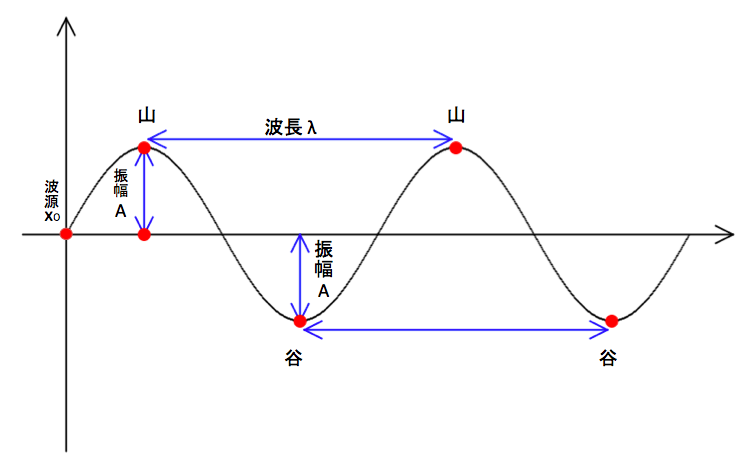
\includegraphics[width=150mm]{../background/lambdasin.png}
 \end{center}
 \caption{波の振幅,波長を示した図.}
 \label{fig:sin}
\end{figure}

\newpage

\section{波の速度と振動数と周期の関係}
1波長分の波が1秒間に発生する回数を振動数$f$[$m$]という.
波の速さ$v$[$m$]は式(\ref{eq:v})と表すことができる.
\begin{eqnarray}
\label{eq:v}
v=fλ
\end{eqnarray}

図\ref{fig:vft}は波の速さ$v$と振動数$f$の関係を示した図である.
\begin{figure}[htbp]
\begin{minipage}[b]{1.0\linewidth}
\centering
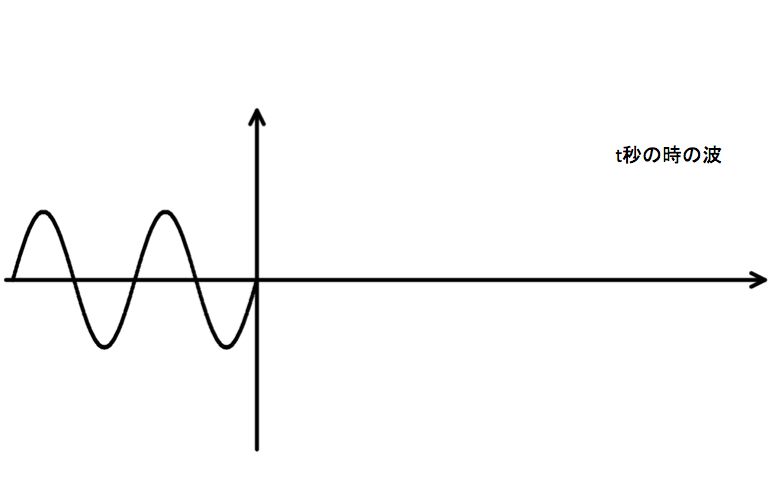
\includegraphics[keepaspectratio, scale=0.42]
  {../background/tminute2.png}
 \subcaption{t秒の時の波.}\label{tminute}
 \end{minipage}
 
\begin{minipage}[b]{1.0\linewidth}
\centering
  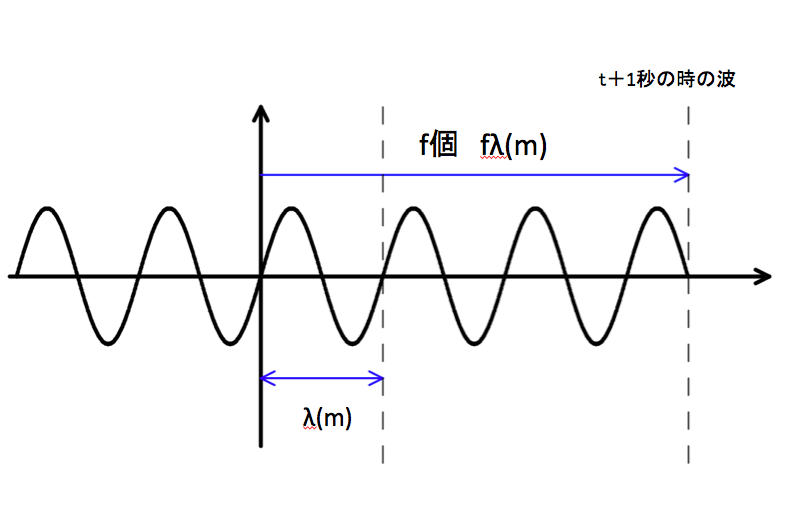
\includegraphics[keepaspectratio, scale=0.42]
  {../background/t+1minute2.png}
 \subcaption{t+1秒の時の波.}\label{t+1minute}
 \end{minipage}
  
  \caption{波の速さv,振動数fの関係を示した図.}
 \label{fig:vft}
\end{figure}

また1波長分の波が発生するまでに要する時間を周期$T$という.
周期$T$と振動数$f$には式(\ref{eq:t})の関係が成り立つ.
\begin{eqnarray}
\label{eq:t}
T = \frac{1}{f}
\end{eqnarray}


\section{ある地点における正弦波の変位の計算方法}
ある地点における正弦波の変位を計算する際には,以下に挙げる要素が必要である.
\begin{enumerate}
 \item 波源からの距離
 \item 波長
 \item 現在の時間と波源が生成された時間との差
 \end{enumerate}
全ての要素を同時に考慮することは難しいので,1-2の要素と3の要素を分けた上で正弦波の変位の計算方法を説明する.

図\ref{fig:dislam}(a)は,ある地点aの変位y\_aと,波源から地点aまでの距離を表したものである.波源から目標地点(点a)までの距離をd1とする.
図\ref{fig:dislam}(b)は\ref{fig:dislam}(a)の距離d1を波長$λ$で割った余りを距離d2とし,波源から距離d2分離れた場所を地点bとして表したものである.




\begin{figure}[htbp]

\begin{minipage}[b]{1.0\linewidth}
\centering
  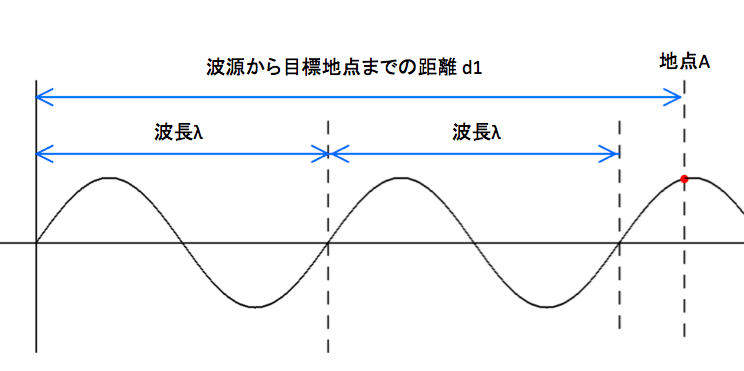
\includegraphics[keepaspectratio, scale=0.45]
  {../background/dislam1.png}
 \subcaption{2つの波が重なっている時.}\label{dislam1}
 \end{minipage}
  
  \begin{minipage}[b]{1.0\linewidth}
\centering
  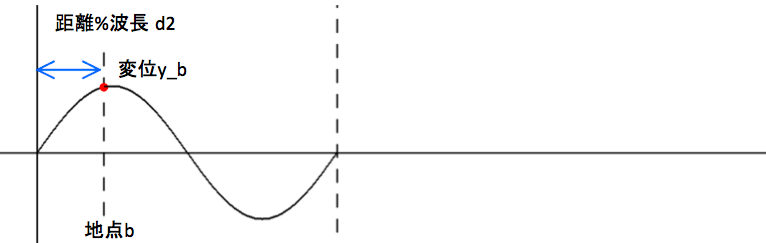
\includegraphics[keepaspectratio, scale=0.45]
  {../background/dislam2.png}
 \subcaption{2つの波が重なった後.}\label{dislam2}
 \end{minipage}
  
  \caption{波源からの距離と波長の値から,ある地点での波の変位を計算する方法.}
 \label{fig:dislam}
\end{figure}











\section{波の独立性と重ね合わせの原理}
教科書P188参考書P104の手法で説明する.


\begin{figure}[htbp]
\begin{minipage}[b]{1.0\linewidth}
\centering
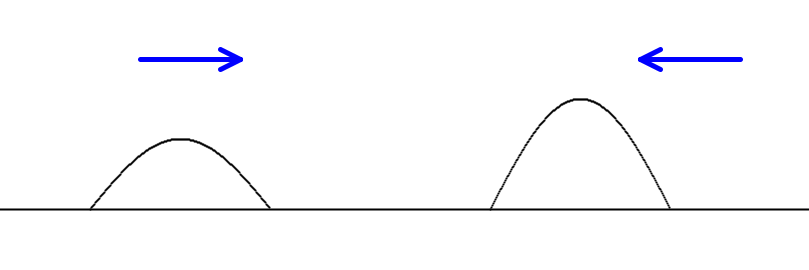
\includegraphics[keepaspectratio, scale=0.45]
  {../background/synwave1.png}
 \subcaption{2つの波が重なる前.}\label{synwave1}
 \end{minipage}
 
\begin{minipage}[b]{1.0\linewidth}
\centering
  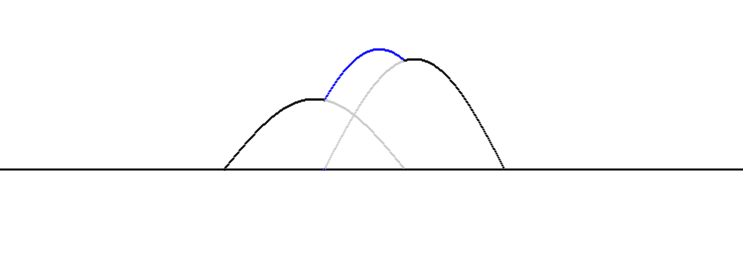
\includegraphics[keepaspectratio, scale=0.45]
  {../background/synwave2.png}
 \subcaption{2つの波が重なっている時.}\label{synwave2}
 \end{minipage}
  
  \begin{minipage}[b]{1.0\linewidth}
\centering
  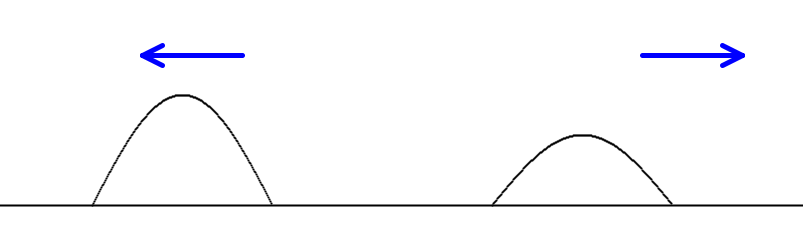
\includegraphics[keepaspectratio, scale=0.45]
  {../background/synwave3.png}
 \subcaption{2つの波が重なった後.}\label{synwave3}
 \end{minipage}
  
  \caption{波の独立性と重ねあわせの原理.}
 \label{fig:synwave}
\end{figure}




\section{反射の法則}
\section{屈折の法則}
\section{回折現象}
\section{ホイヘンスの原理}
上の3つの現象をホイヘンスの原理によって説明する方法を示す.




















\begin{comment}




\chapter{物理的背景}
\section{分子動力学法}
分子動力学法は運動方程式を解く事によって,粒子の振る舞いを解析する手法である\cite{MD}.ニュートンの運動方程式はエネルギー保存則を満たすため,エネルギーが保存される集団において用いられる.
\subsection{Verlet法}
Verlet法は分子動力学法における粒子の座標を逐次的に求める方法であり,式(\ref{eq:verlet})のように表される.


\begin{eqnarray}
\label{eq:verlet}
r(t+h)=2r(t)-r(t-h)+\frac{h^2}{m}f(t)
\end{eqnarray}
ここで,$r(t)$は時刻$t$における粒子の座標,$f(t)$は時刻$t$における粒子に加わっている力,$h$は微小時間,$m$は粒子の質量を表している.
式(\ref{eq:verlet})は,時刻$t$における粒子の座標,時刻$t-h$における粒子の座標,時刻$t$における粒子に加わっている力,粒子の質量の4つの要素から,時刻$t+h$における粒子の座標が求まることを表している.
粒子に加わっている力を常に決定することができれば,Verlet法を継続的に用いることが可能であり,逐次的に粒子の座標を決定し続けることができる.
また,粒子を動かすために速度が必要そうだが,この手法では速度を必要としないという特徴がある.この手法はニュートンの運動方程式から導出されるため,エネルギーが保存される系で有効である.


\subsection{導出}
時刻$t+h$における粒子の座標$r(t+h)$にテイラー展開を行うと式(\ref{eq:verlet2})ができる.

\begin{eqnarray}
\label{eq:verlet2}
r(t+h)=r(t)+h\frac{dr(t)}{dt}+\frac{h^2}{2!}\frac{d^2r(t)}{dt^2}+\frac{h^3}{3!}\frac{d^3r(t)}{dt^3}+...
\end{eqnarray}

$h$は微小時間のため$h^3$以上の項を無視すると
\begin{eqnarray}
\label{eq:verlet5}
r(t+h)=r(t)+h\frac{dr(t)}{dt}+\frac{h^2}{2!}\frac{d^2r(t)}{dt^2}
\end{eqnarray}

$h$を$-h$に置き換えると
\begin{eqnarray}
\label{eq:verlet6}
r(t-h)=r(t)-h\frac{dr(t)}{dt}+\frac{h^2}{2!}\frac{d^2r(t)}{dt^2}
\end{eqnarray}

式(\ref{eq:verlet5})と式(\ref{eq:verlet6})を足し合わせ$r(t+h)$について移項させると式(\ref{eq:verlet3})ができる.

\begin{eqnarray}
\label{eq:verlet3}
r(t+h)=2r(t)-r(t-h)-h^2\frac{d^2r(t)}{dt^2}
\end{eqnarray}

ここでニュートンの運動方程式について考える.$v(t)$を時刻$t$の速度,$r(t)$を時刻$t$の位置とすると式(\ref{eq:newton})ができる.
\begin{eqnarray}
\label{eq:newton}
v(t)=\frac{dr(t)}{dt}
\end{eqnarray}
また,式(\ref{eq:newton})より時刻$t$における加速度$a(t)$は
\begin{eqnarray}
a(t)=\frac{d^2r(t)}{dt^2}
\end{eqnarray}
ここで$f(t)$を時刻$t$に作用する力,$m$を質量とするとニュートンの運動方程式は式(\ref{eq:newton2})となる.
\begin{eqnarray}
\label{eq:newton2}
f(t)=m\frac{d^2r(t)}{dt^2}
\end{eqnarray}
移項させると
\begin{eqnarray}
\label{eq:newton4}
\frac{f(t)}{m}=\frac{d^2r(t)}{dt^2}
\end{eqnarray}

式(\ref{eq:newton4})を式(\ref{eq:verlet3})にを代入すると式(\ref{eq:newton3})となりVerlet法が導出される.
\begin{eqnarray}
\label{eq:newton3}
r(t+h)=2r(t)-r(t-h)+\frac{h^2}{m}f(t)
\end{eqnarray}


\section{Lennard-Jonesポテンシャル}
Lennard-Jonesポテンシャルとは2体間での相互作用ポテンシャルエネルギーを経験則的に表したモデルである\cite{akahon}.$ψ$をポテンシャルエネルギー,$R$を原子間距離,$A$,$B$は任意の定数とすると式(\ref{eq:lennard})のように表される.
\begin{eqnarray}
\label{eq:lennard}
\psi(R)=A\bigg(\frac{1}{R}\bigg)^{12}+B\bigg(\frac{1}{R}\bigg)^6
\end{eqnarray}
式(\ref{eq:lennard})は縦軸をポテンシャルエネルギー,横軸を粒子間距離とすると図\ref{fig:lennard}のような概形になる.


ポテンシャルエネルギーの理解には,安定した状態からずれるとエネルギーが生じるという考え方が適切である.
図\ref{fig:lennard}では極小点が平衡原子間距離であり,双方の粒子が安定した状態であると言える.
原子間距離が安定状態より近くなれば,急激にエネルギーが上がる.これは近づくことで原子同士の影響力が増大するからである.
逆に,安定状態より遠くなると,エネルギーは緩やかに上がっていき,ある高さで上昇が止まる.これは原子同士の影響力が減少するからである.
これに加えて,原子に作用する力について考えていく.ポテンシャルエネルギーを距離で微分することにより作用する力が求まる
.図\ref{fig:lennard}の傾きに注目すると,
平衡原子間距離は極小点であり傾きは0のため力が作用しない.
また,距離が近くなれば傾きは急激に負の値をとり斥力が生まれる.逆に,遠くなれば傾きは正の値をとり引力が生まれるが,傾きが徐々に0に近づくため力が弱まっていく.このように図\ref{fig:lennard}のような概形のポテンシャルエネルギーは,バネのような振る舞いをすることがわかる.
\begin{figure}[htbp]
 \begin{center}
  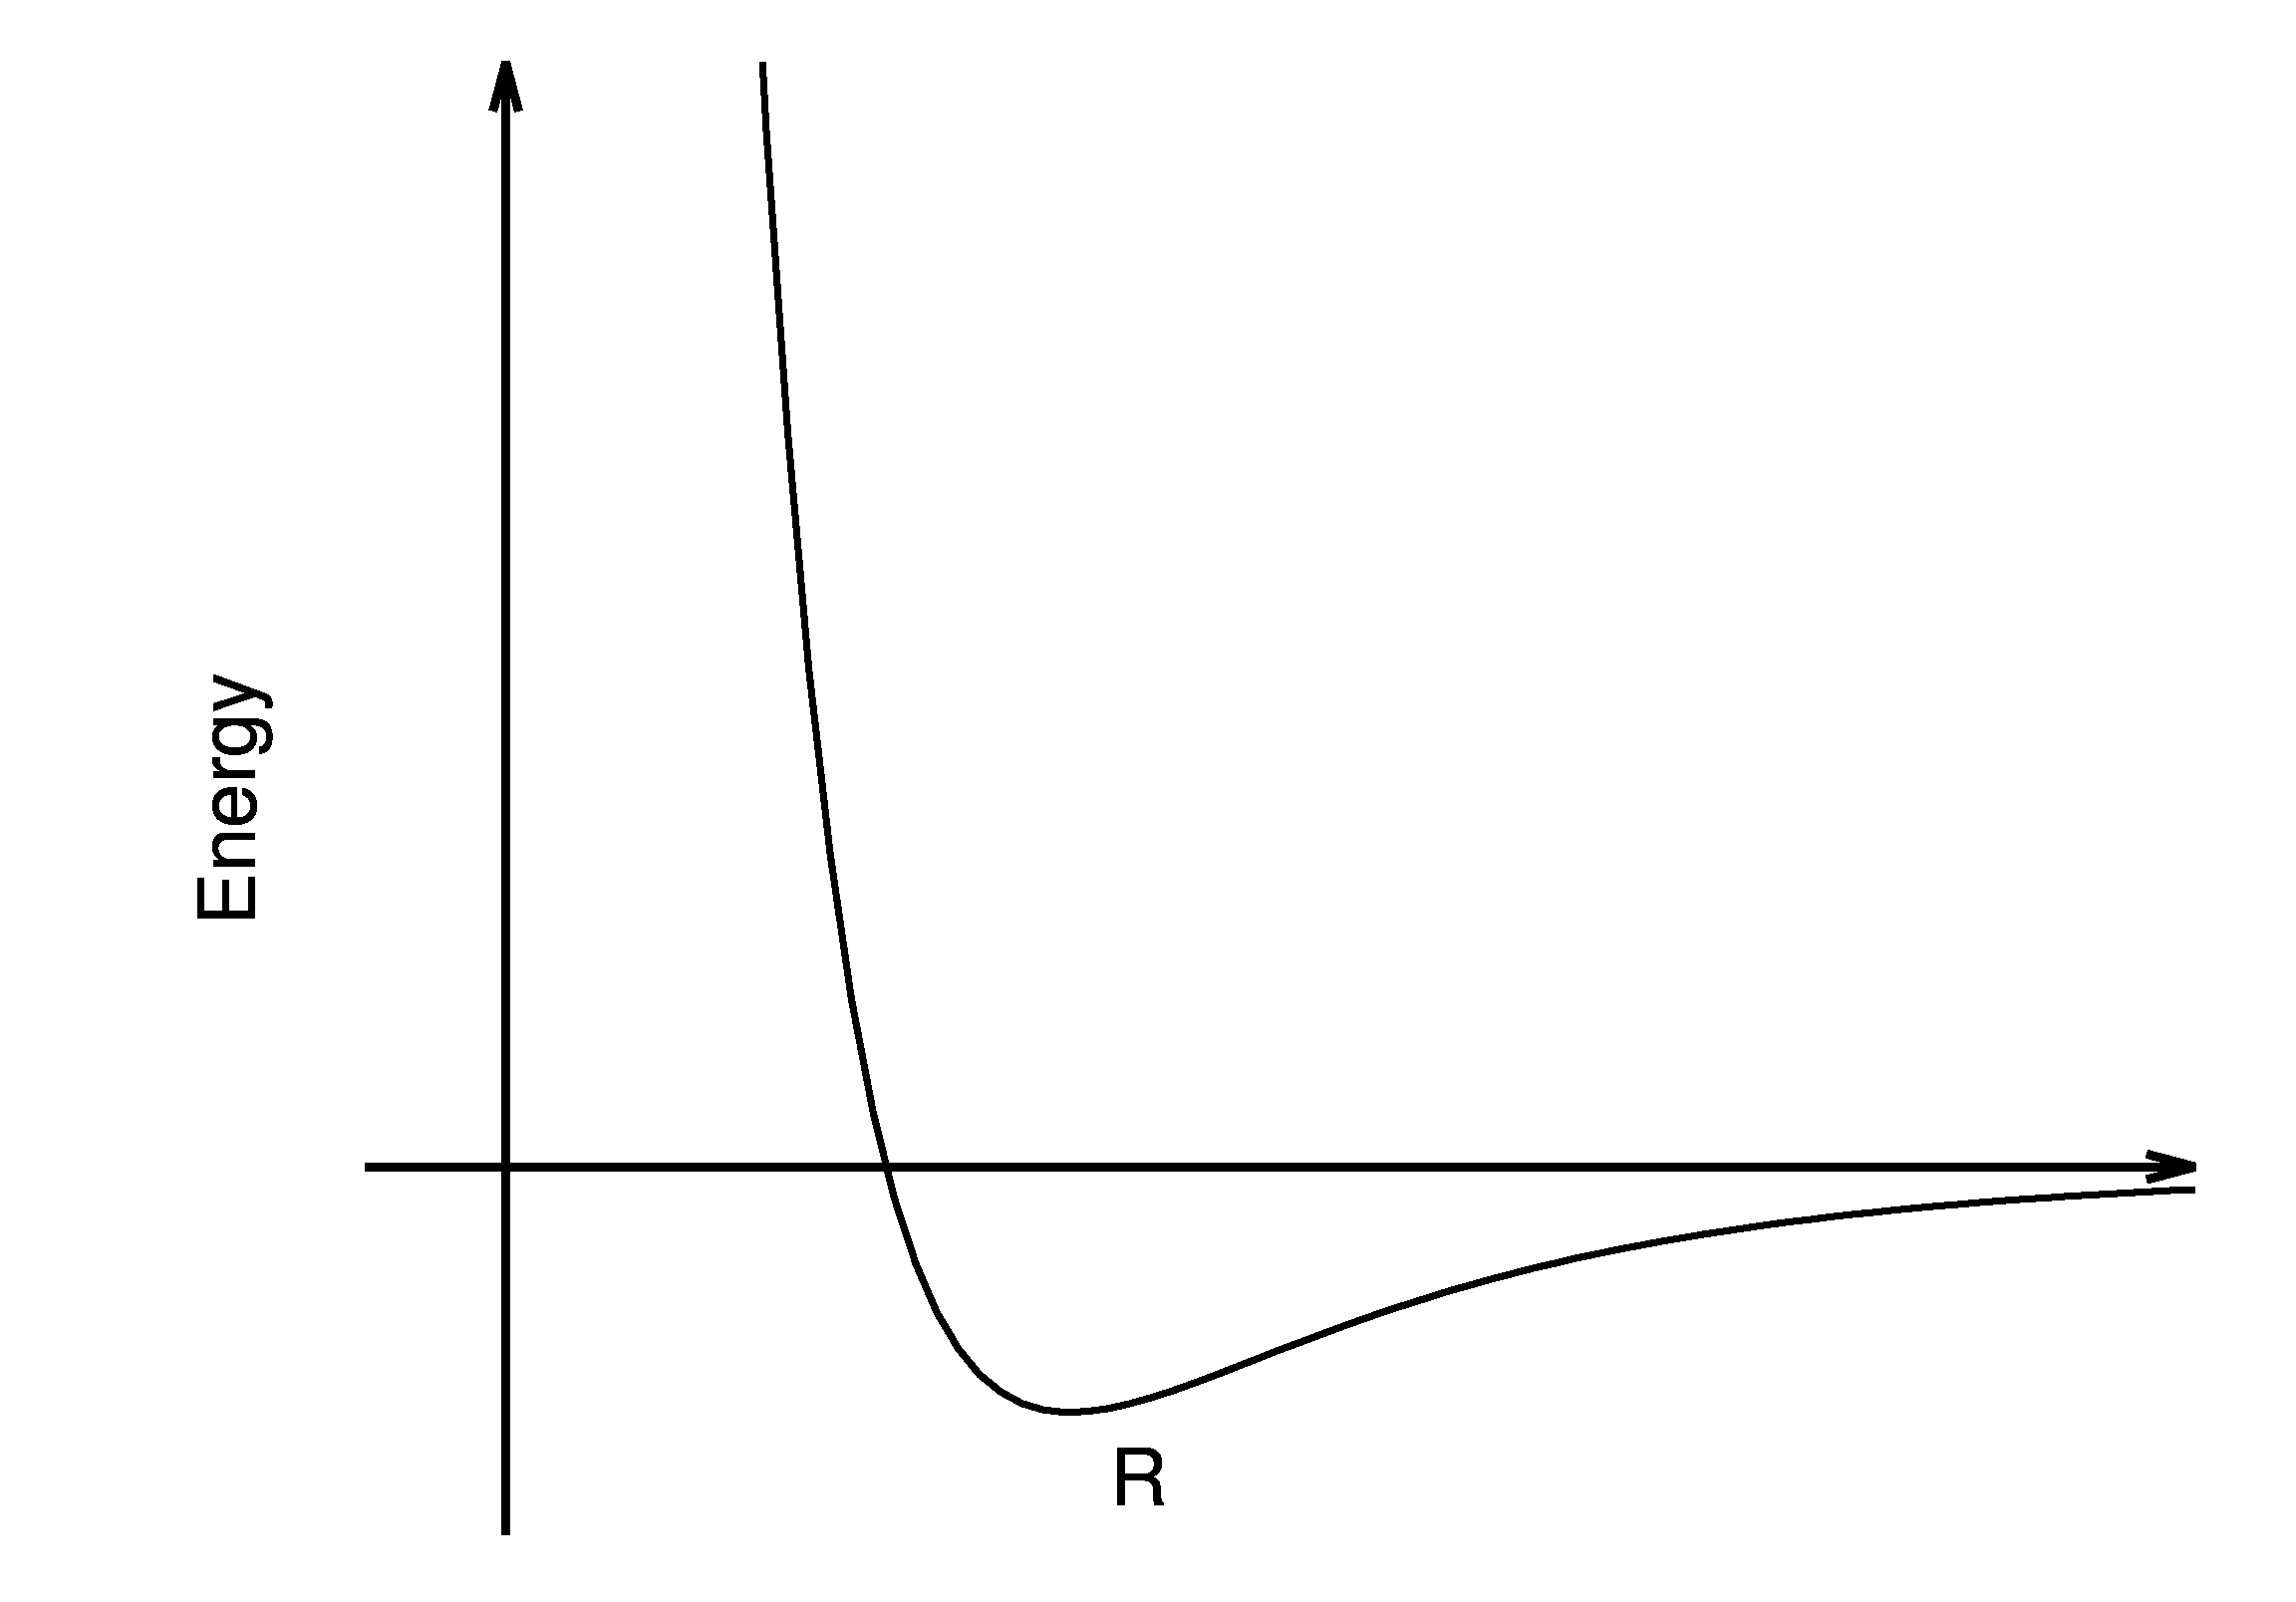
\includegraphics[width=150mm]{../intro/lennard.png}
 \end{center}
 \caption{Lennard-Jonesポテンシャル.}
 \label{fig:lennard}
\end{figure}

\end{comment}%物理学的基礎知識
\chapter{結果}
本章では,波の各性質をプログラムによって視覚化した実行結果を記述する.いずれのプログラムもJavaScriptへ変換可能であり,Webブラウザ上で動作させることが可能である.

\section{円形波の位相変位を視覚化したプログラム}
図\ref{fig:4wave}は指定した複数の点源から生成される円形波の位相変位をシミュレーションし,視覚化を行うプログラムである.
このプログラムにはdrawモードとcheckモードという2つのモードが実装されており,drawモードからcheckモードに移行するにはCキー(checkの頭文字).checkモードからdrawモードに移行するときはDキー(drawの頭文字)を押せばよい.


\begin{figure}[htbp]
 \begin{center}
  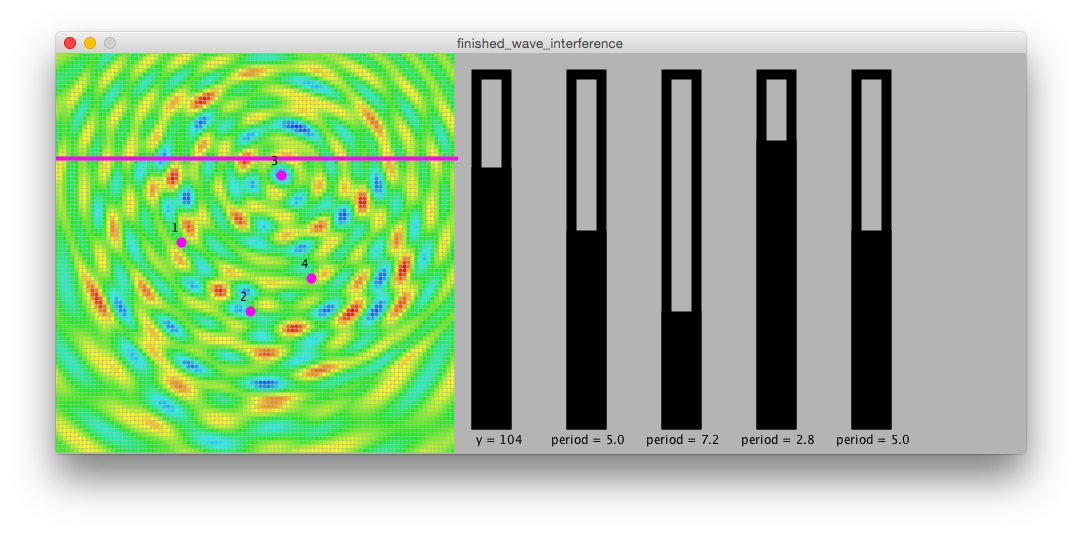
\includegraphics[width=\linewidth]{../result/4wave.png}
 \end{center}
 \caption{波の位相変位を視覚化したプログラムの画面.}
 \label{fig:4wave}
\end{figure}






\subsection{drawモード}
このモードは波源から生じる円形波を描写するモードである. プログラム起動時の画面が図\ref{fig:0wave}である.
\begin{figure}[htbp]
 \begin{center}
  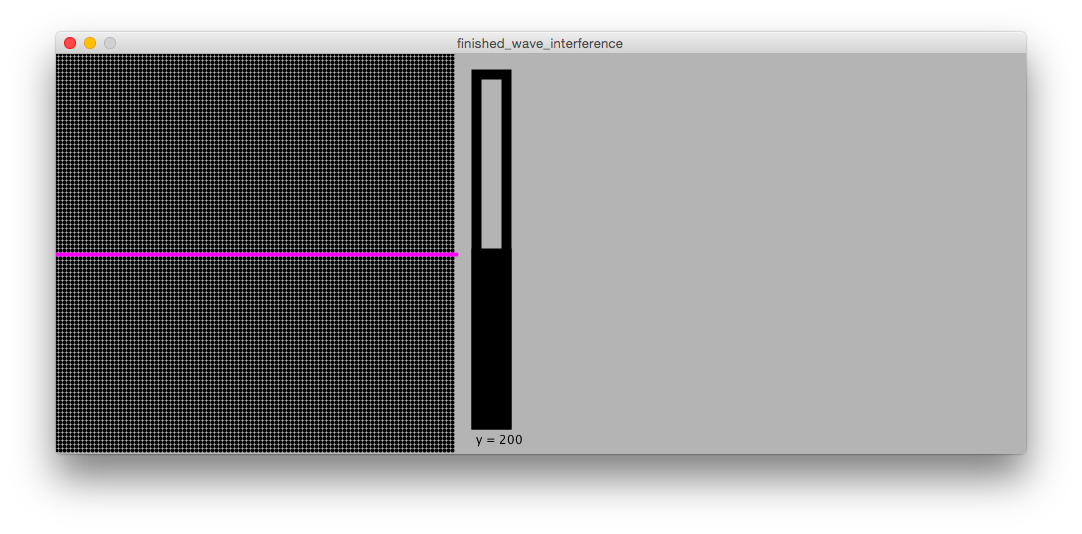
\includegraphics[width=\linewidth]{../result/0wave.png}
 \end{center}
 \caption{プログラム起動時の画面.}
 \label{fig:0wave}
\end{figure}

画面左側の黒い領域が波を描写する領域,画面右側にはcheckモードで確認するy座標の位置を操作できるスライダーが配置されている(いきなりスライダーと言っていいのか?). 
図\ref{fig:0wave}の状態で黒い領域上のいずれかの場所をクリックすると,クリックされた座標に波源が生成される.波源が生成されたあと,画面右側にはその波源の周期を変更できるスライダーが生成される.

図\ref{fig:wave}は1つの波源を生成した後,周期をスライダーによって変更した様子である.
\begin{figure}[htbp]
 \begin{center}
  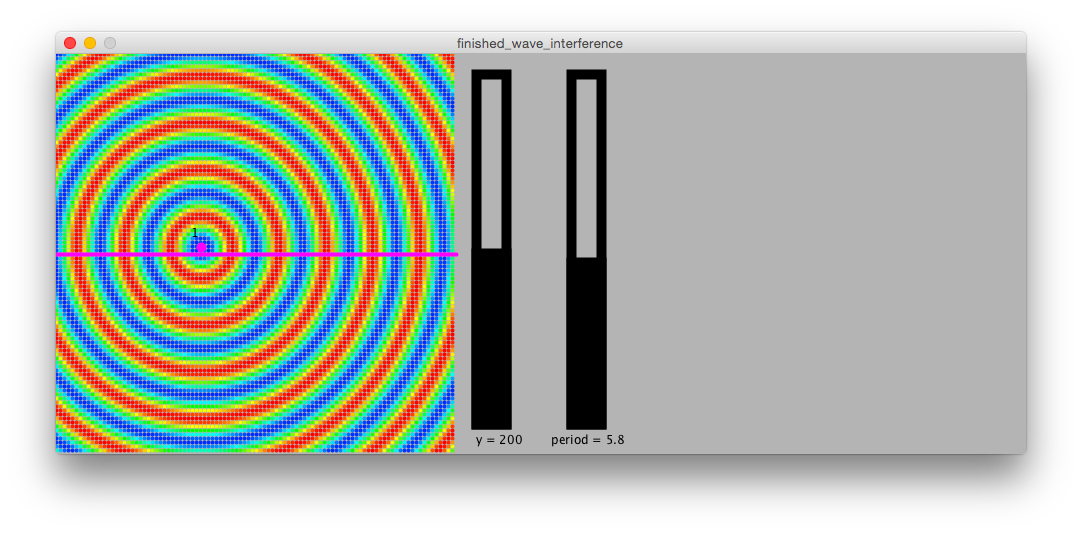
\includegraphics[width=\linewidth]{../result/wave.png}
 \end{center}
 \caption{1つの波の周期をスライダーで変更した画面.}
 \label{fig:wave}
\end{figure}

\newpage
スライダーが周期を変更できる状態で
Lキー(lambdaの頭文字)を押すと,図\ref{fig:wavechangelambda}のように波の波長を変更できるスライダーに変化する.周期を変更するスライダーに戻したい場合はPキー(periodの頭文字)を押せばよい.

\begin{figure}[htbp]
 \begin{center}
  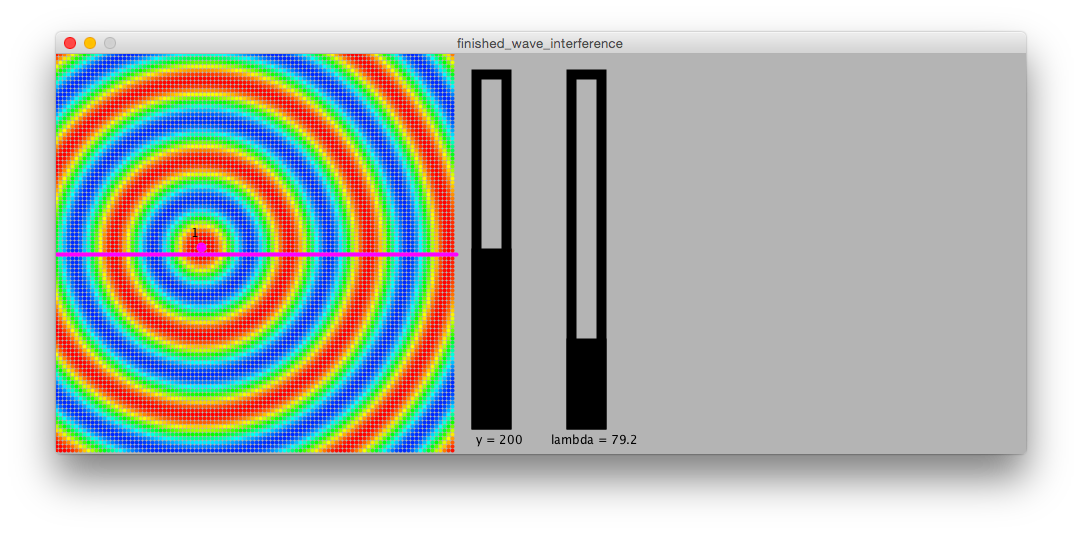
\includegraphics[width=\linewidth]{../result/wavechangelambda.png}
 \end{center}
 \caption{波長を変更できるスライダーに変化させた時の画面.}
 \label{fig:wavechangelambda}
\end{figure}

波源は図\ref{fig:5wave}のように5個まで生成できる.

\begin{figure}[htbp]
 \begin{center}
  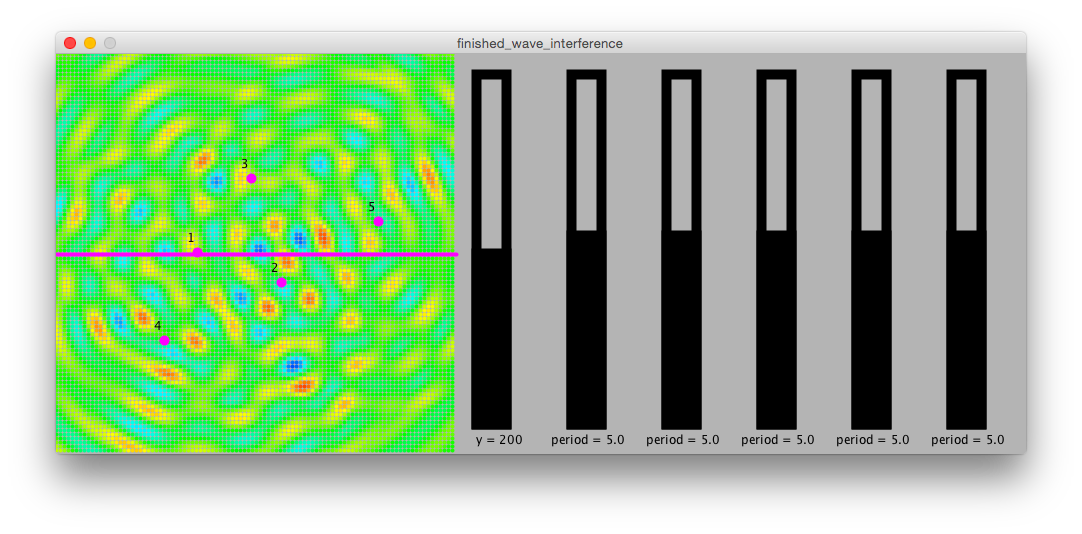
\includegraphics[width=\linewidth]{../result/5wave.png}
 \end{center}
 \caption{波源を5個生成した時の画面.}
 \label{fig:5wave}
\end{figure}

\newpage
\subsection{checkモード}
このモードはdrawモードに描写されている赤い線上の位相変位をリアルタイムに視覚化するモードである.同時刻,同座標で周期,波長が同一な波を生成し,波を生成して360フレーム目の状態をdrawモード,checkモードでそれぞれ描写したのが図\ref{fig:compare}(\subref{drawmode}),(\subref{checkmode})である.(ほんまに一致しているか先生に見てもらう)


\begin{figure}[htbp]
\begin{minipage}[b]{1.0\linewidth}
\centering
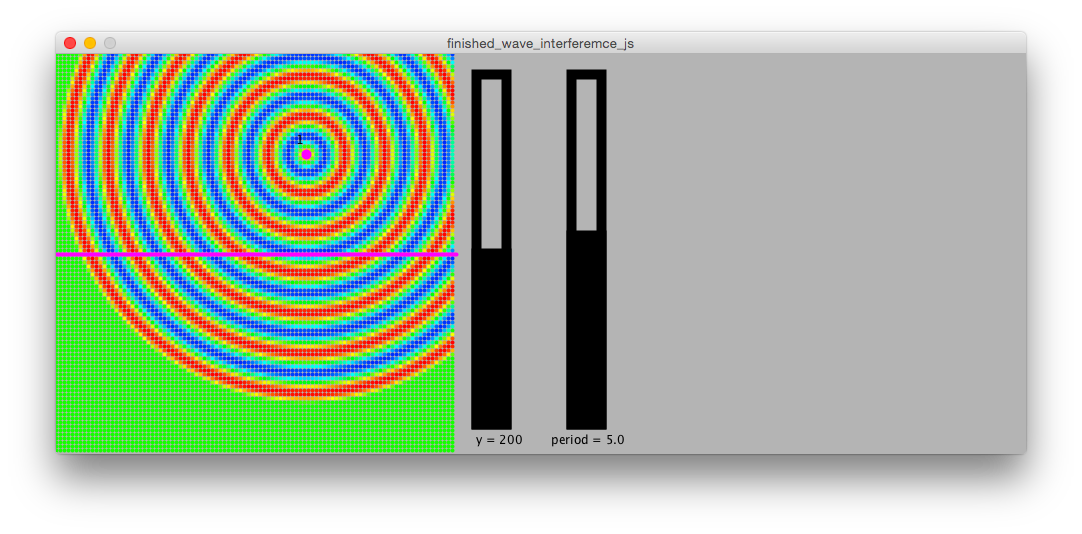
\includegraphics[keepaspectratio, scale=0.40]
  {../result/drawmode.png}
 \subcaption{drawモード.}\label{drawmode}
 \end{minipage}
 
\begin{minipage}[b]{1.0\linewidth}
\centering
  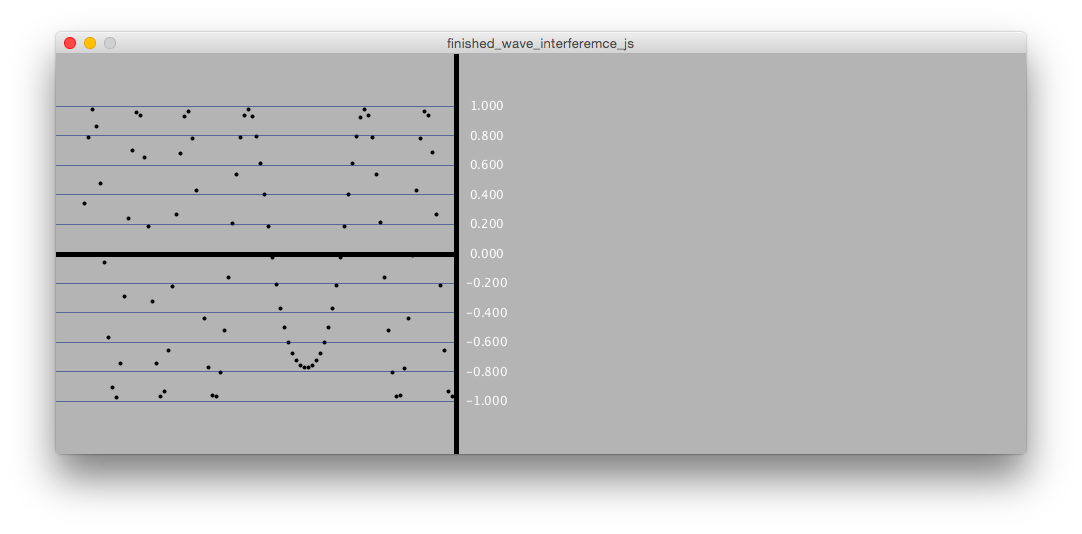
\includegraphics[keepaspectratio, scale=0.40]
  {../result/checkmode.png}
 \subcaption{checkモード.}\label{checkmode}
 \end{minipage}
  
  \caption{周期5.0,波長40.0の波が生成されてから360フレーム目のdrawモード,checkモードの画面.}
 \label{fig:compare}
\end{figure}



\newpage
\section{波の回折現象を視覚化したプログラム}
\section{波の反射を視覚化したプログラム}
出来なかった理由はプログラム解説の章で解説していいのか?
\section{波の屈折を視覚化したプログラム}























\begin{comment}

%図\ref{fig:MDprogram}は本研究で作成したVerlet法とLennard-Jonesポテンシャルを用いて粒子の振る舞いをシミュレーションし,視覚化を行うプログラムである.
%Processingで作成しているが,JavaScriptへ変換する事によってWebブラウザ上で動作させる事が可能である.
%左の枠内に複数の粒子モデルが描画され,それらが枠内を動き回る.また,粒子の色を速度によって青から赤に変化させてエネルギーの推移をわかりやすくし,マウスカーソルで粒子をクリックしドラッグする\chapter{結果}
本章では,波の各性質をプログラムによって視覚化した実行結果を記述する.いずれのプログラムもJavaScriptへ変換可能であり,Webブラウザ上で動作させることが可能である.

\section{円形波の位相変位を視覚化したプログラム}
図\ref{fig:4wave}は指定した複数の点源から生成される円形波の位相変位をシミュレーションし,視覚化を行うプログラムである.
このプログラムにはdrawモードとcheckモードという2つのモードが実装されており,drawモードからcheckモードに移行するにはCキー(checkの頭文字).checkモードからdrawモードに移行するときはDキー(drawの頭文字)を押せばよい.


\begin{figure}[htbp]
 \begin{center}
  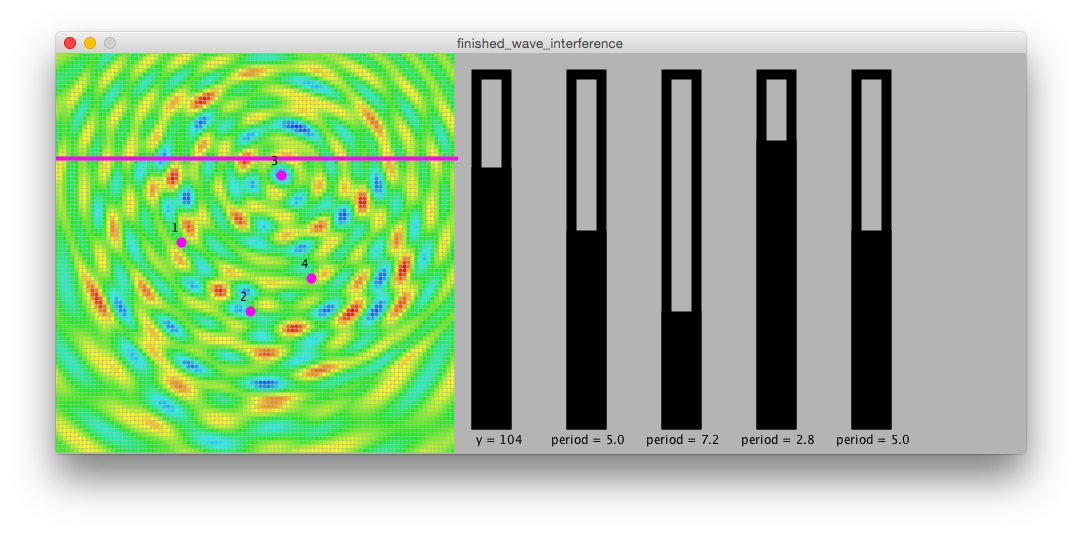
\includegraphics[width=\linewidth]{../result/4wave.png}
 \end{center}
 \caption{波の位相変位を視覚化したプログラムの画面.}
 \label{fig:4wave}
\end{figure}






\subsection{drawモード}
このモードは波源から生じる円形波を描写するモードである. プログラム起動時の画面が図\ref{fig:0wave}である.
\begin{figure}[htbp]
 \begin{center}
  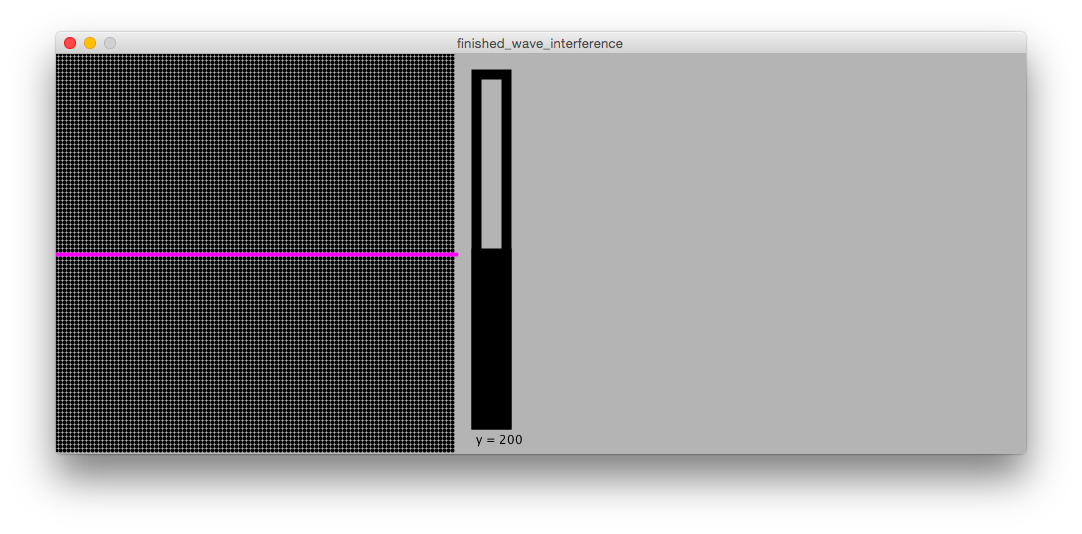
\includegraphics[width=\linewidth]{../result/0wave.png}
 \end{center}
 \caption{プログラム起動時の画面.}
 \label{fig:0wave}
\end{figure}

画面左側の黒い領域が波を描写する領域,画面右側にはcheckモードで確認するy座標の位置を操作できるスライダーが配置されている(いきなりスライダーと言っていいのか?). 
図\ref{fig:0wave}の状態で黒い領域上のいずれかの場所をクリックすると,クリックされた座標に波源が生成される.波源が生成されたあと,画面右側にはその波源の周期を変更できるスライダーが生成される.

図\ref{fig:wave}は1つの波源を生成した後,周期をスライダーによって変更した様子である.
\begin{figure}[htbp]
 \begin{center}
  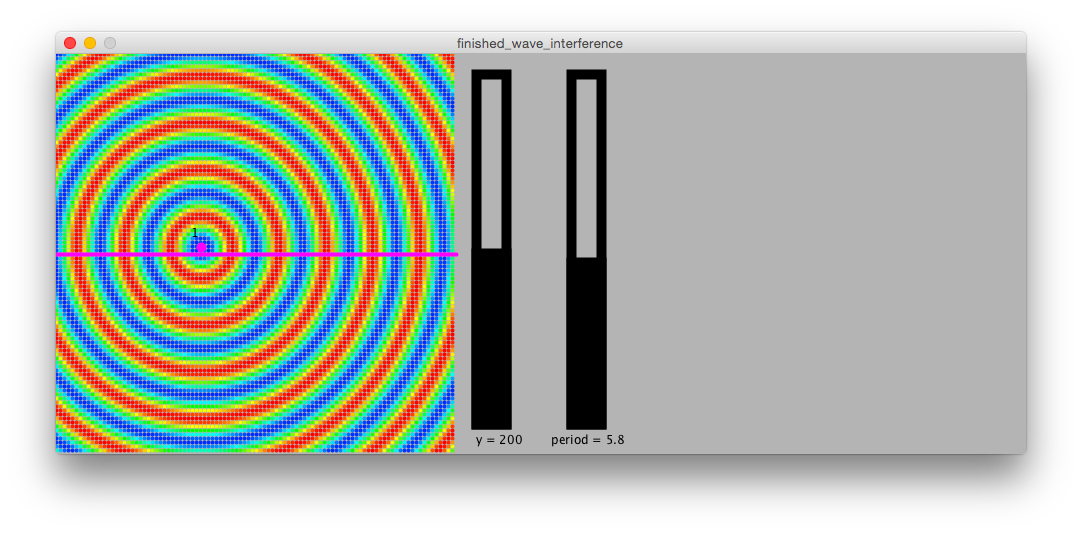
\includegraphics[width=\linewidth]{../result/wave.png}
 \end{center}
 \caption{1つの波の周期をスライダーで変更した画面.}
 \label{fig:wave}
\end{figure}

\newpage
スライダーが周期を変更できる状態で
Lキー(lambdaの頭文字)を押すと,図\ref{fig:wavechangelambda}のように波の波長を変更できるスライダーに変化する.周期を変更するスライダーに戻したい場合はPキー(periodの頭文字)を押せばよい.

\begin{figure}[htbp]
 \begin{center}
  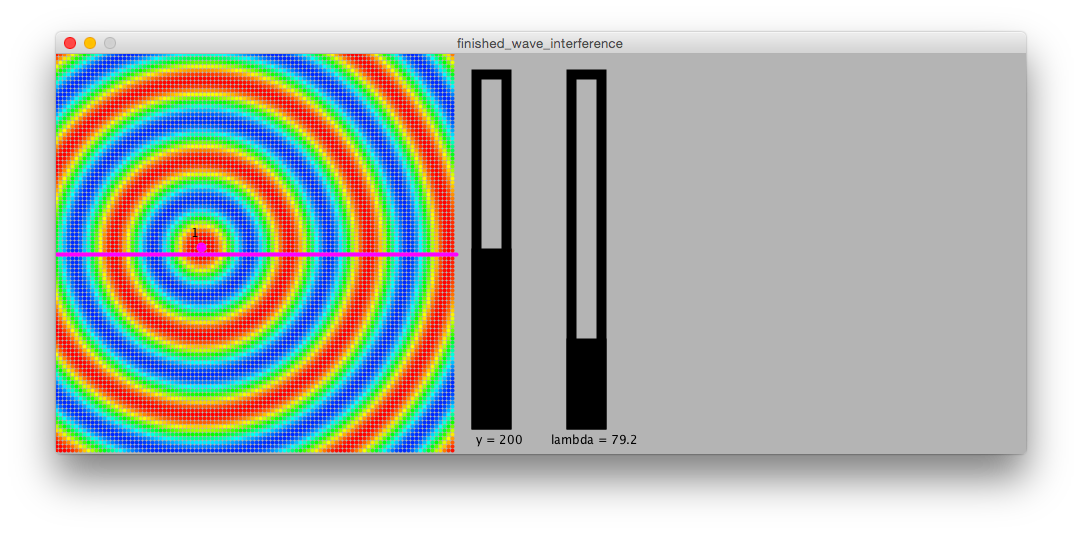
\includegraphics[width=\linewidth]{../result/wavechangelambda.png}
 \end{center}
 \caption{波長を変更できるスライダーに変化させた時の画面.}
 \label{fig:wavechangelambda}
\end{figure}

波源は図\ref{fig:5wave}のように5個まで生成できる.

\begin{figure}[htbp]
 \begin{center}
  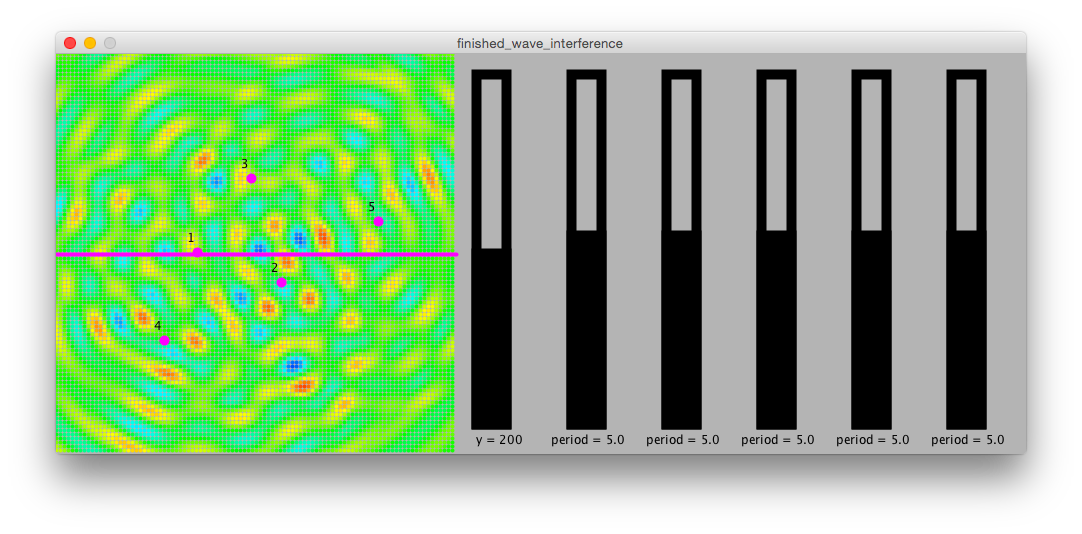
\includegraphics[width=\linewidth]{../result/5wave.png}
 \end{center}
 \caption{波源を5個生成した時の画面.}
 \label{fig:5wave}
\end{figure}

\newpage
\subsection{checkモード}
このモードはdrawモードに描写されている赤い線上の位相変位をリアルタイムに視覚化するモードである.同時刻,同座標で周期,波長が同一な波を生成し,波を生成して360フレーム目の状態をdrawモード,checkモードでそれぞれ描写したのが図\ref{fig:compare}(\subref{drawmode}),(\subref{checkmode})である.(ほんまに一致しているか先生に見てもらう)


\begin{figure}[htbp]
\begin{minipage}[b]{1.0\linewidth}
\centering
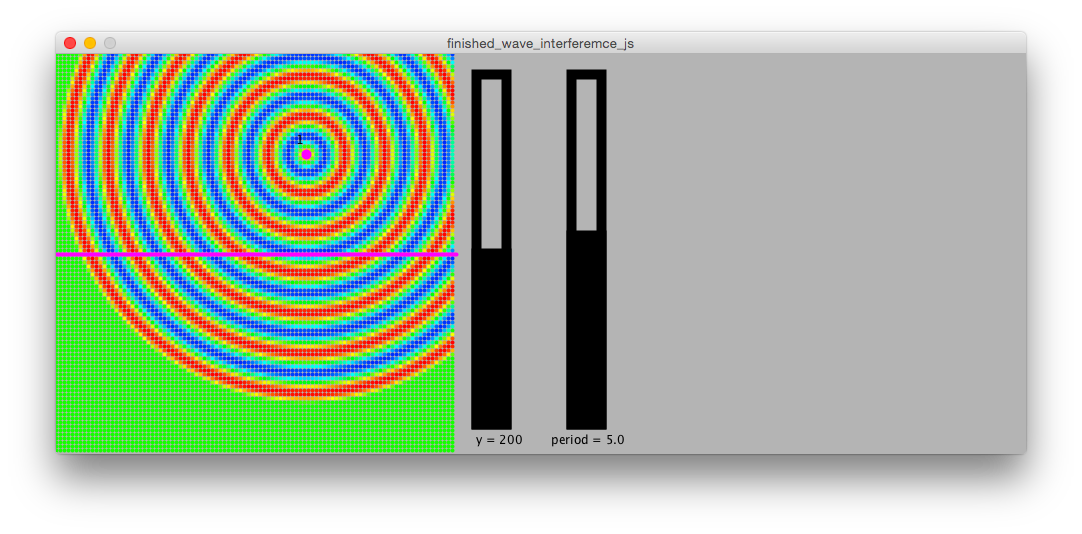
\includegraphics[keepaspectratio, scale=0.40]
  {../result/drawmode.png}
 \subcaption{drawモード.}\label{drawmode}
 \end{minipage}
 
\begin{minipage}[b]{1.0\linewidth}
\centering
  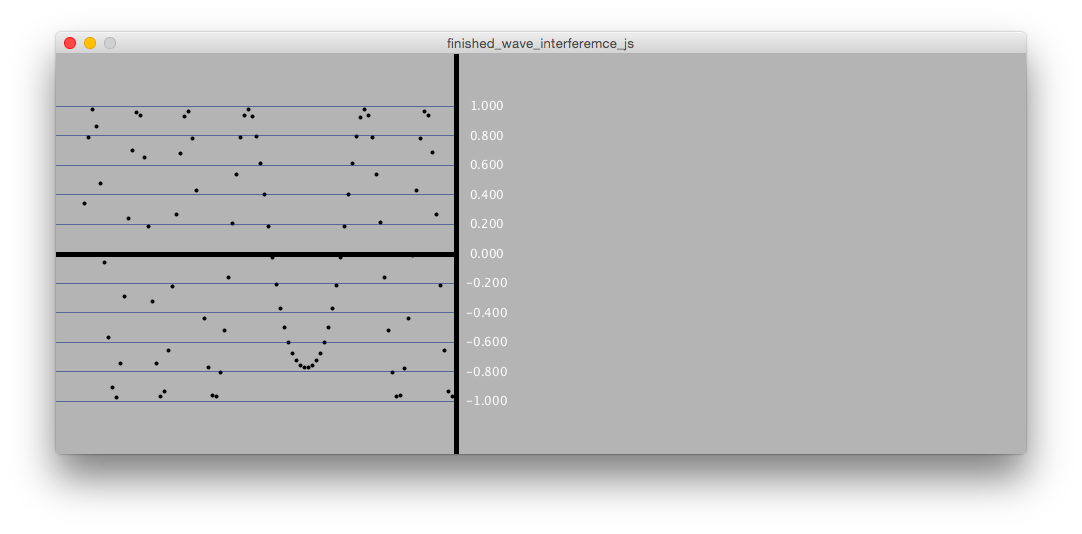
\includegraphics[keepaspectratio, scale=0.40]
  {../result/checkmode.png}
 \subcaption{checkモード.}\label{checkmode}
 \end{minipage}
  
  \caption{周期5.0,波長40.0の波が生成されてから360フレーム目のdrawモード,checkモードの画面.}
 \label{fig:compare}
\end{figure}



\newpage
\section{波の回折現象を視覚化したプログラム}
\section{波の反射を視覚化したプログラム}
出来なかった理由はプログラム解説の章で解説していいのか?
\section{波の屈折を視覚化したプログラム}























\begin{comment}

%図\ref{fig:MDprogram}は本研究で作成したVerlet法とLennard-Jonesポテンシャルを用いて粒子の振る舞いをシミュレーションし,視覚化を行うプログラムである.
%Processingで作成しているが,JavaScriptへ変換する事によってWebブラウザ上で動作させる事が可能である.
%左の枠内に複数の粒子モデルが描画され,それらが枠内を動き回る.また,粒子の色を速度によって青から赤に変化させてエネルギーの推移をわかりやすくし,マウスカーソルで粒子をクリックしドラッグする\chapter{結果}
本章では,波の各性質をプログラムによって視覚化した実行結果を記述する.いずれのプログラムもJavaScriptへ変換可能であり,Webブラウザ上で動作させることが可能である.

\section{円形波の位相変位を視覚化したプログラム}
図\ref{fig:4wave}は指定した複数の点源から生成される円形波の位相変位をシミュレーションし,視覚化を行うプログラムである.
このプログラムにはdrawモードとcheckモードという2つのモードが実装されており,drawモードからcheckモードに移行するにはCキー(checkの頭文字).checkモードからdrawモードに移行するときはDキー(drawの頭文字)を押せばよい.


\begin{figure}[htbp]
 \begin{center}
  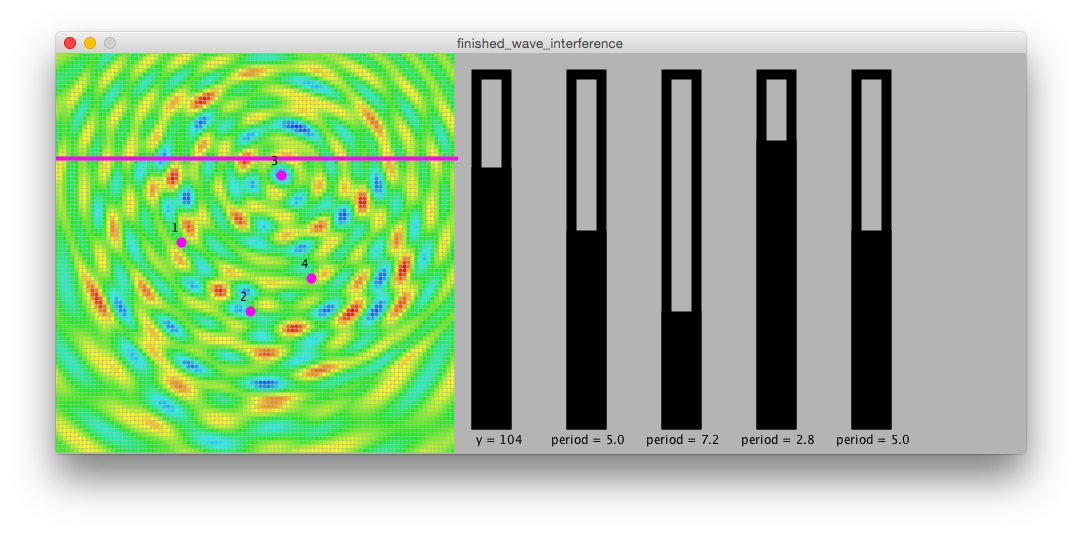
\includegraphics[width=\linewidth]{../result/4wave.png}
 \end{center}
 \caption{波の位相変位を視覚化したプログラムの画面.}
 \label{fig:4wave}
\end{figure}






\subsection{drawモード}
このモードは波源から生じる円形波を描写するモードである. プログラム起動時の画面が図\ref{fig:0wave}である.
\begin{figure}[htbp]
 \begin{center}
  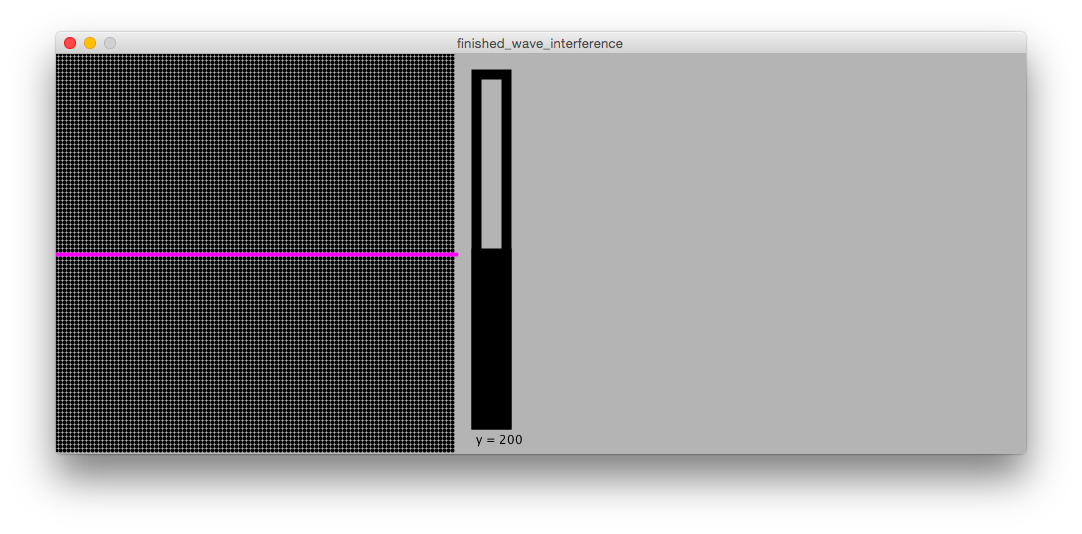
\includegraphics[width=\linewidth]{../result/0wave.png}
 \end{center}
 \caption{プログラム起動時の画面.}
 \label{fig:0wave}
\end{figure}

画面左側の黒い領域が波を描写する領域,画面右側にはcheckモードで確認するy座標の位置を操作できるスライダーが配置されている(いきなりスライダーと言っていいのか?). 
図\ref{fig:0wave}の状態で黒い領域上のいずれかの場所をクリックすると,クリックされた座標に波源が生成される.波源が生成されたあと,画面右側にはその波源の周期を変更できるスライダーが生成される.

図\ref{fig:wave}は1つの波源を生成した後,周期をスライダーによって変更した様子である.
\begin{figure}[htbp]
 \begin{center}
  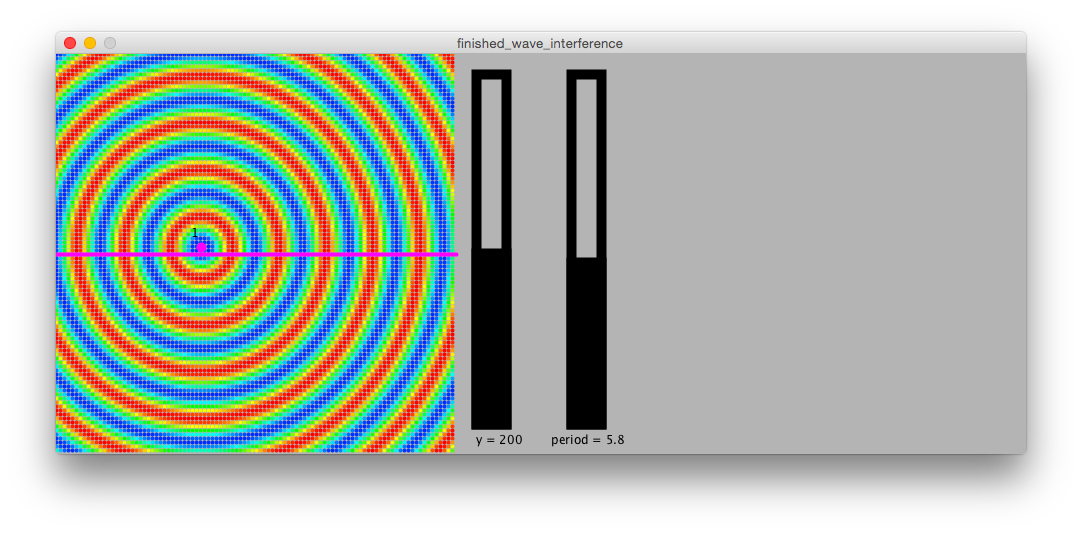
\includegraphics[width=\linewidth]{../result/wave.png}
 \end{center}
 \caption{1つの波の周期をスライダーで変更した画面.}
 \label{fig:wave}
\end{figure}

\newpage
スライダーが周期を変更できる状態で
Lキー(lambdaの頭文字)を押すと,図\ref{fig:wavechangelambda}のように波の波長を変更できるスライダーに変化する.周期を変更するスライダーに戻したい場合はPキー(periodの頭文字)を押せばよい.

\begin{figure}[htbp]
 \begin{center}
  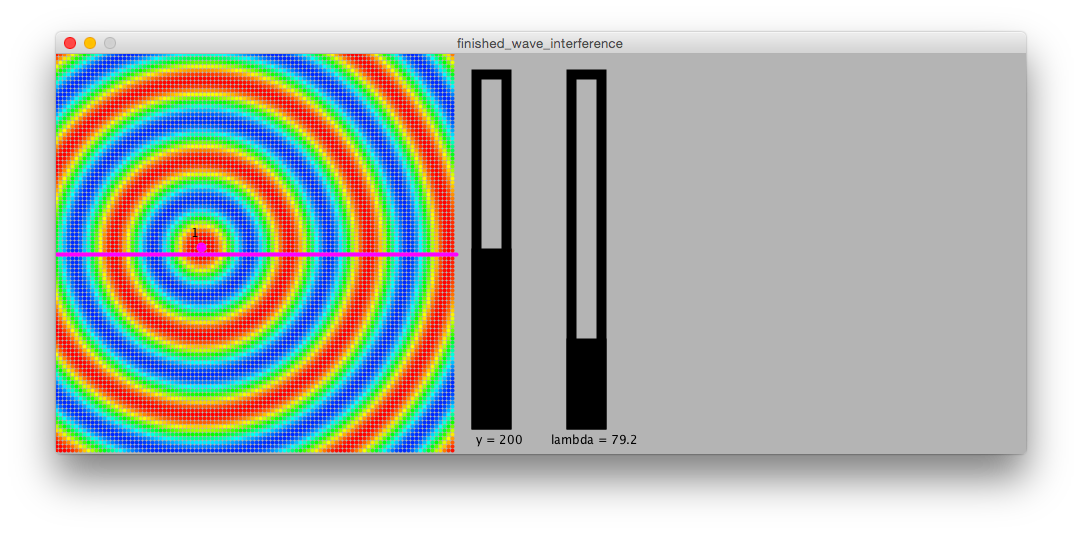
\includegraphics[width=\linewidth]{../result/wavechangelambda.png}
 \end{center}
 \caption{波長を変更できるスライダーに変化させた時の画面.}
 \label{fig:wavechangelambda}
\end{figure}

波源は図\ref{fig:5wave}のように5個まで生成できる.

\begin{figure}[htbp]
 \begin{center}
  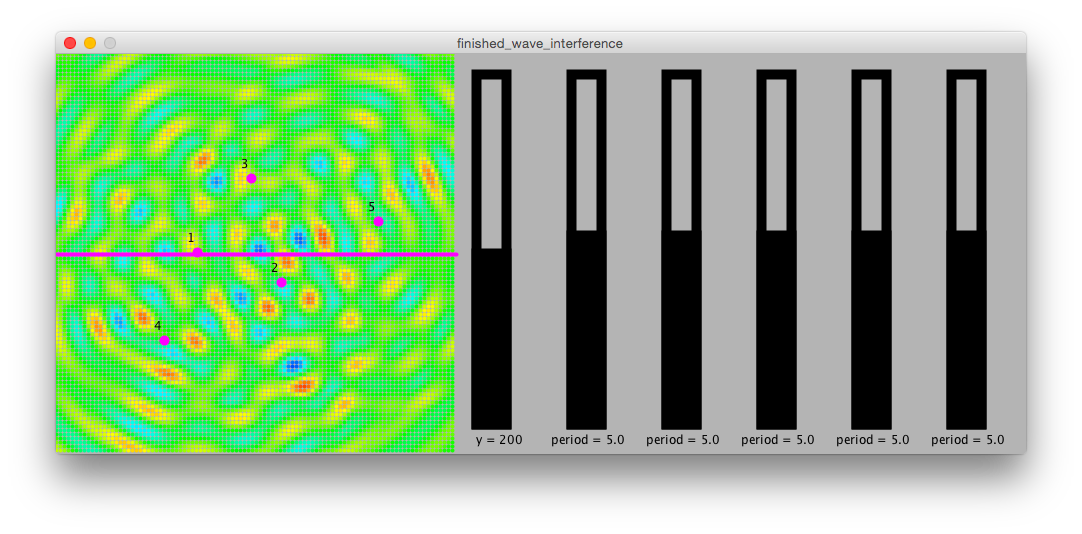
\includegraphics[width=\linewidth]{../result/5wave.png}
 \end{center}
 \caption{波源を5個生成した時の画面.}
 \label{fig:5wave}
\end{figure}

\newpage
\subsection{checkモード}
このモードはdrawモードに描写されている赤い線上の位相変位をリアルタイムに視覚化するモードである.同時刻,同座標で周期,波長が同一な波を生成し,波を生成して360フレーム目の状態をdrawモード,checkモードでそれぞれ描写したのが図\ref{fig:compare}(\subref{drawmode}),(\subref{checkmode})である.(ほんまに一致しているか先生に見てもらう)


\begin{figure}[htbp]
\begin{minipage}[b]{1.0\linewidth}
\centering
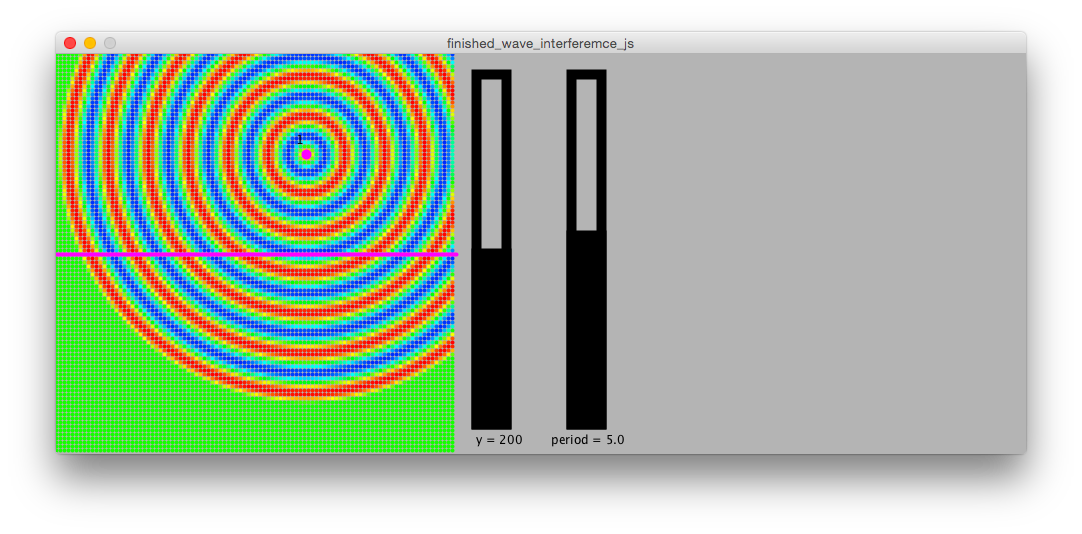
\includegraphics[keepaspectratio, scale=0.40]
  {../result/drawmode.png}
 \subcaption{drawモード.}\label{drawmode}
 \end{minipage}
 
\begin{minipage}[b]{1.0\linewidth}
\centering
  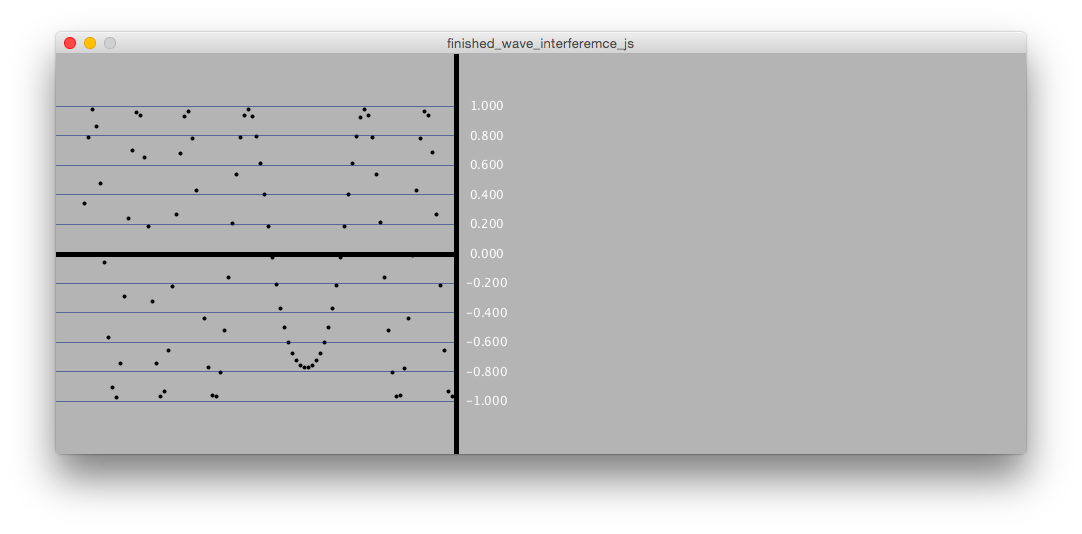
\includegraphics[keepaspectratio, scale=0.40]
  {../result/checkmode.png}
 \subcaption{checkモード.}\label{checkmode}
 \end{minipage}
  
  \caption{周期5.0,波長40.0の波が生成されてから360フレーム目のdrawモード,checkモードの画面.}
 \label{fig:compare}
\end{figure}



\newpage
\section{波の回折現象を視覚化したプログラム}
\section{波の反射を視覚化したプログラム}
出来なかった理由はプログラム解説の章で解説していいのか?
\section{波の屈折を視覚化したプログラム}























\begin{comment}

%図\ref{fig:MDprogram}は本研究で作成したVerlet法とLennard-Jonesポテンシャルを用いて粒子の振る舞いをシミュレーションし,視覚化を行うプログラムである.
%Processingで作成しているが,JavaScriptへ変換する事によってWebブラウザ上で動作させる事が可能である.
%左の枠内に複数の粒子モデルが描画され,それらが枠内を動き回る.また,粒子の色を速度によって青から赤に変化させてエネルギーの推移をわかりやすくし,マウスカーソルで粒子をクリックしドラッグする\input{result.tex}
%事によって好きな方向に力を加える事ができる.
%右側には2本のスライダーがあり,粒子の数とVerlet法の時間刻みを調整できる.
%キー入力により状態を変更することができ,Sキーで凝固状態,Fキーで粒子に加わる力を視覚化した状態,Rキーで粒子のリセットを行うことができる.

\newpage
\begin{figure}[htbp]
 \begin{center}
  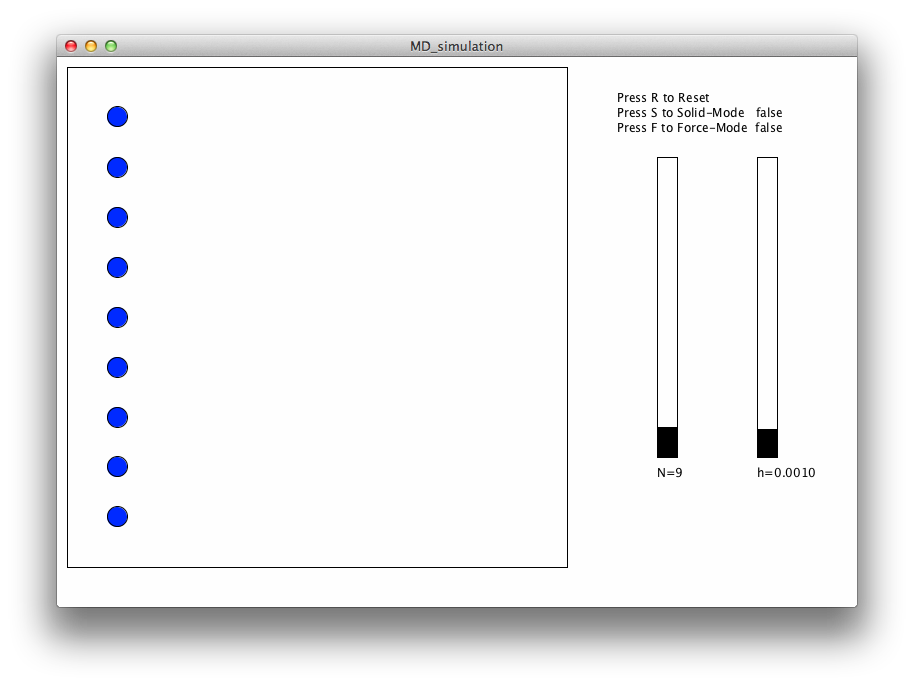
\includegraphics[width=150mm]{../implement/MDprogram.png} %implementのフォルダにあるpng画像
 \end{center}
 \caption{分子動力学法視覚化プログラム.}
 \label{fig:MDprogram}
\end{figure}

\newpage

図\ref{fig:cluster}は粒子クラスタの移動を表しており,それぞれの粒子のクラスタとしての振る舞いを視認することができる.
スライダーで粒子の数を変更しマウスで力を加えることによって,このようなクラスタを好きなようにシミュレーションできる.
\begin{figure}[htbp]
 \begin{center}
  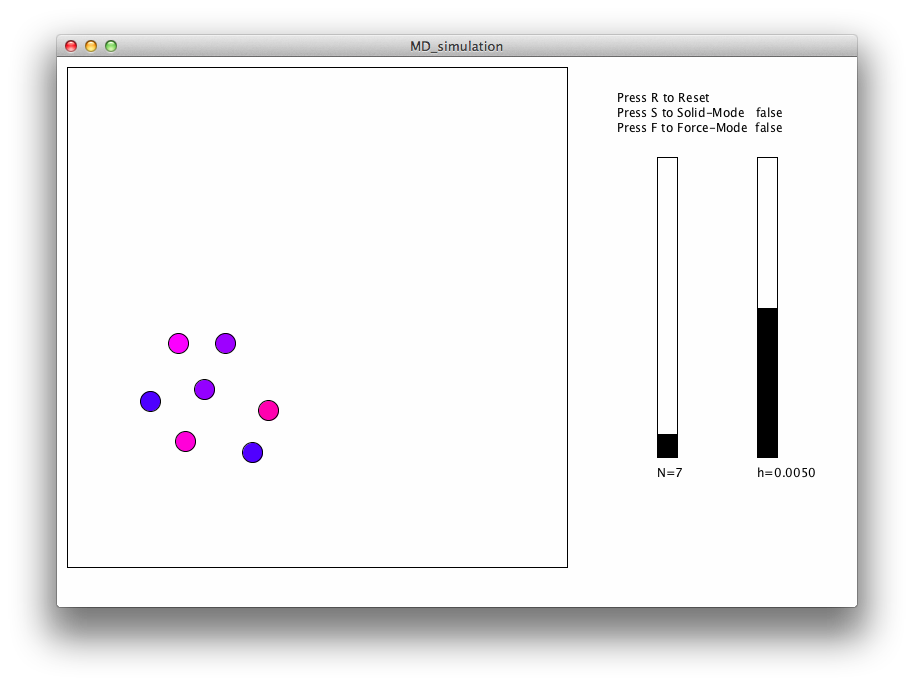
\includegraphics[width=150mm]{../result/cluster_picture.png}
 \end{center}
 \caption{クラスタの移動.}
 \label{fig:cluster}
\end{figure}


\newpage

図\ref{fig:solid}は凝固状態にしてしばらく実行し続けた結果であり,粒子が下の方に集まっていることが確認できる.これは粒子に下向きの力を継続的に加えて擬似的に凝固の現象を表現している.
これにより,粒子が自由に動き回る液体や気体の状態から,個体に移り変わる凝固現象の様子を確認できる.


\begin{figure}[htbp]
 \begin{center}
  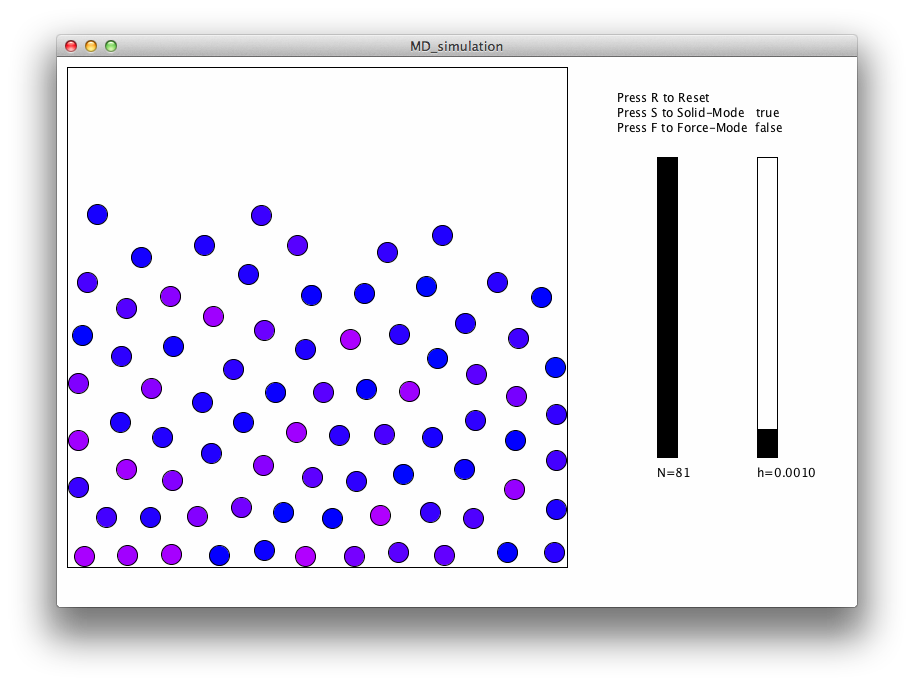
\includegraphics[width=150mm]{../implement/solid_mode.png}
 \end{center}
 \caption{凝固状態.}
 \label{fig:solid}
\end{figure}

\newpage

図\ref{fig:force}は粒子に加わる力を視覚化した状態であり,それぞれの粒子の中心から線が伸びている.
この線は長さが力の大きさ,向きが力の向きと対応しており力の加わり方をリアルタイムで把握することができる.
それぞれの粒子が力のパラメータを持っており,それらはシュミレーションの中で瞬時に変化していくため,値の確認は困難である.
しかし,この視覚化のおかげでそれぞれの粒子にかかる力を直感的に確認できる.

\begin{figure}[htbp]
 \begin{center}
  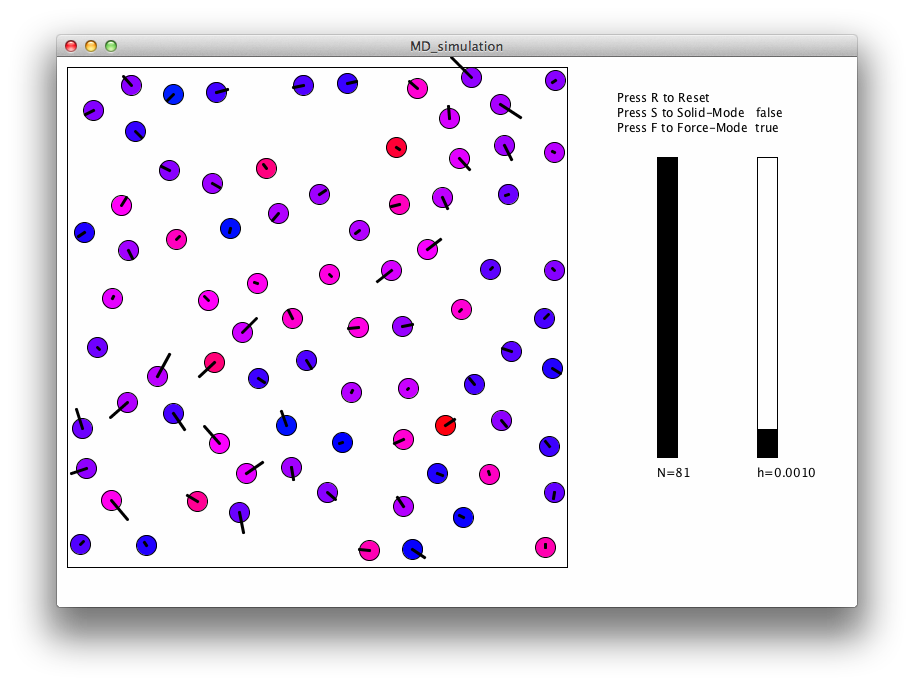
\includegraphics[width=150mm]{../implement/force_mode.png}
 \end{center}
 \caption{粒子に加わる力を視覚化した状態.}
 \label{fig:force}
\end{figure}


\end{comment}

%事によって好きな方向に力を加える事ができる.
%右側には2本のスライダーがあり,粒子の数とVerlet法の時間刻みを調整できる.
%キー入力により状態を変更することができ,Sキーで凝固状態,Fキーで粒子に加わる力を視覚化した状態,Rキーで粒子のリセットを行うことができる.

\newpage
\begin{figure}[htbp]
 \begin{center}
  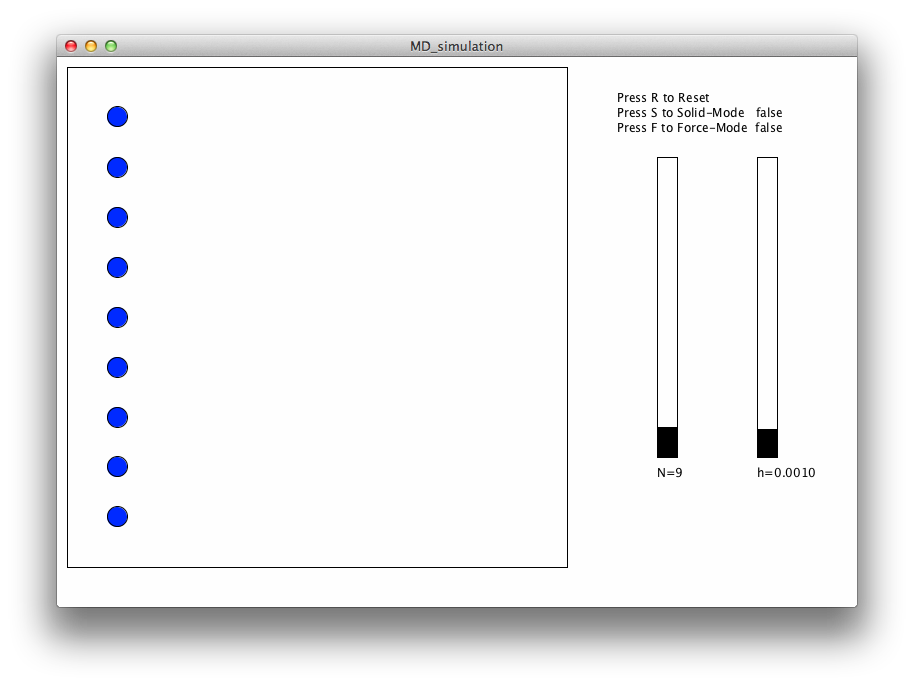
\includegraphics[width=150mm]{../implement/MDprogram.png} %implementのフォルダにあるpng画像
 \end{center}
 \caption{分子動力学法視覚化プログラム.}
 \label{fig:MDprogram}
\end{figure}

\newpage

図\ref{fig:cluster}は粒子クラスタの移動を表しており,それぞれの粒子のクラスタとしての振る舞いを視認することができる.
スライダーで粒子の数を変更しマウスで力を加えることによって,このようなクラスタを好きなようにシミュレーションできる.
\begin{figure}[htbp]
 \begin{center}
  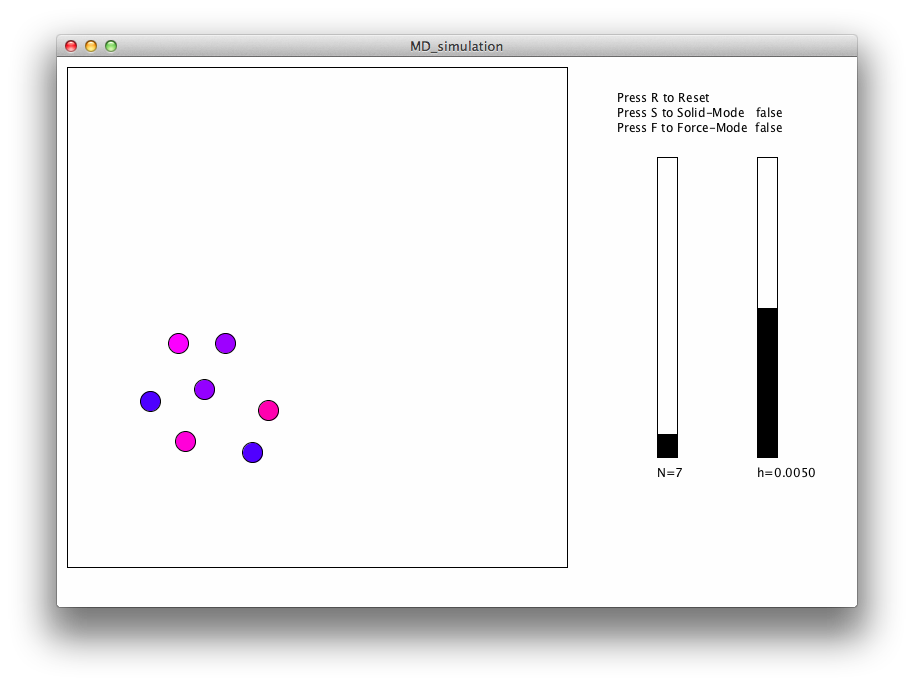
\includegraphics[width=150mm]{../result/cluster_picture.png}
 \end{center}
 \caption{クラスタの移動.}
 \label{fig:cluster}
\end{figure}


\newpage

図\ref{fig:solid}は凝固状態にしてしばらく実行し続けた結果であり,粒子が下の方に集まっていることが確認できる.これは粒子に下向きの力を継続的に加えて擬似的に凝固の現象を表現している.
これにより,粒子が自由に動き回る液体や気体の状態から,個体に移り変わる凝固現象の様子を確認できる.


\begin{figure}[htbp]
 \begin{center}
  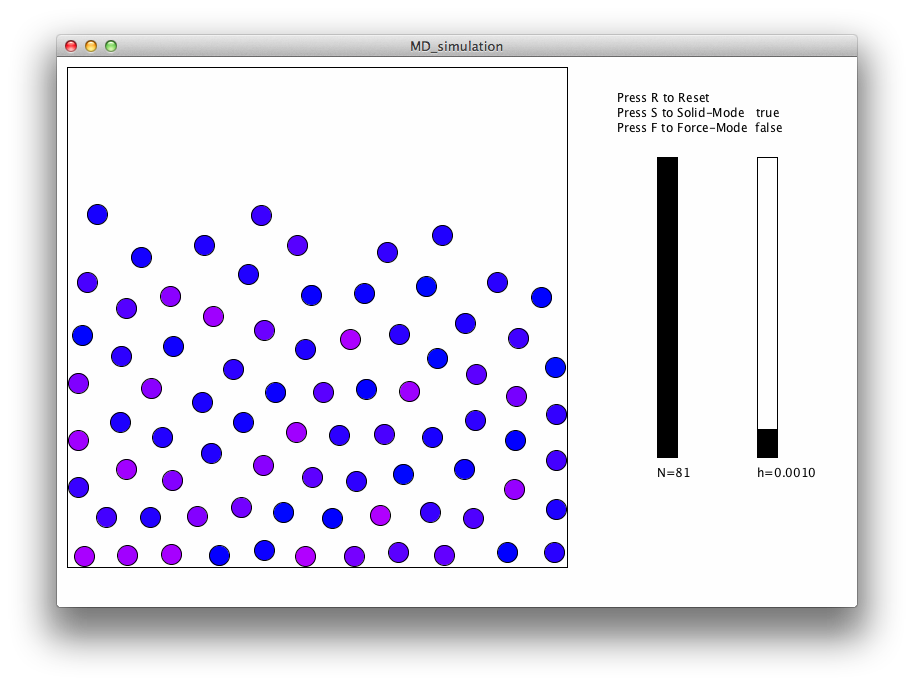
\includegraphics[width=150mm]{../implement/solid_mode.png}
 \end{center}
 \caption{凝固状態.}
 \label{fig:solid}
\end{figure}

\newpage

図\ref{fig:force}は粒子に加わる力を視覚化した状態であり,それぞれの粒子の中心から線が伸びている.
この線は長さが力の大きさ,向きが力の向きと対応しており力の加わり方をリアルタイムで把握することができる.
それぞれの粒子が力のパラメータを持っており,それらはシュミレーションの中で瞬時に変化していくため,値の確認は困難である.
しかし,この視覚化のおかげでそれぞれの粒子にかかる力を直感的に確認できる.

\begin{figure}[htbp]
 \begin{center}
  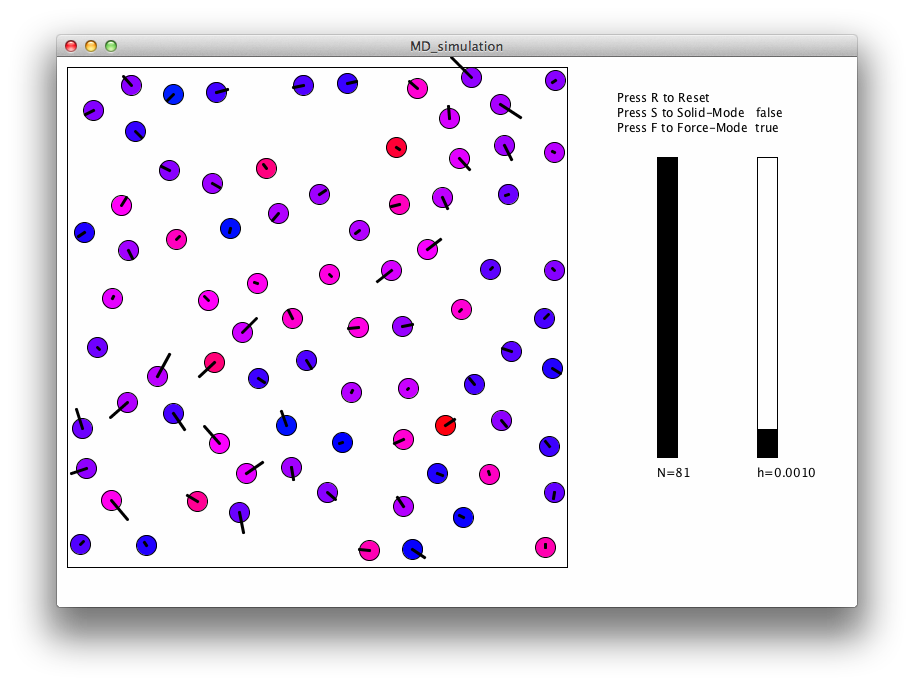
\includegraphics[width=150mm]{../implement/force_mode.png}
 \end{center}
 \caption{粒子に加わる力を視覚化した状態.}
 \label{fig:force}
\end{figure}


\end{comment}

%事によって好きな方向に力を加える事ができる.
%右側には2本のスライダーがあり,粒子の数とVerlet法の時間刻みを調整できる.
%キー入力により状態を変更することができ,Sキーで凝固状態,Fキーで粒子に加わる力を視覚化した状態,Rキーで粒子のリセットを行うことができる.

\newpage
\begin{figure}[htbp]
 \begin{center}
  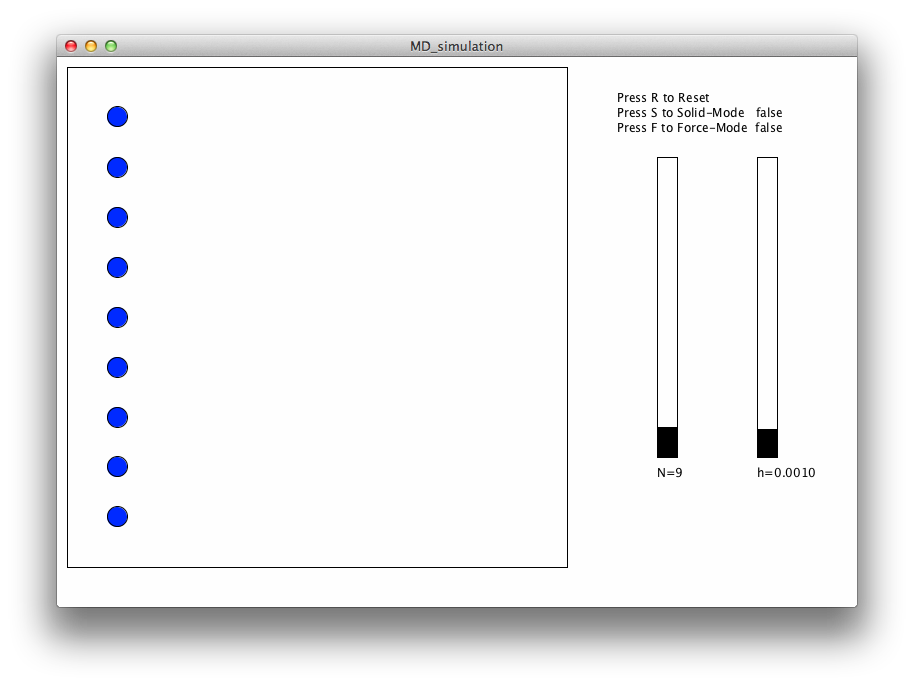
\includegraphics[width=150mm]{../implement/MDprogram.png} %implementのフォルダにあるpng画像
 \end{center}
 \caption{分子動力学法視覚化プログラム.}
 \label{fig:MDprogram}
\end{figure}

\newpage

図\ref{fig:cluster}は粒子クラスタの移動を表しており,それぞれの粒子のクラスタとしての振る舞いを視認することができる.
スライダーで粒子の数を変更しマウスで力を加えることによって,このようなクラスタを好きなようにシミュレーションできる.
\begin{figure}[htbp]
 \begin{center}
  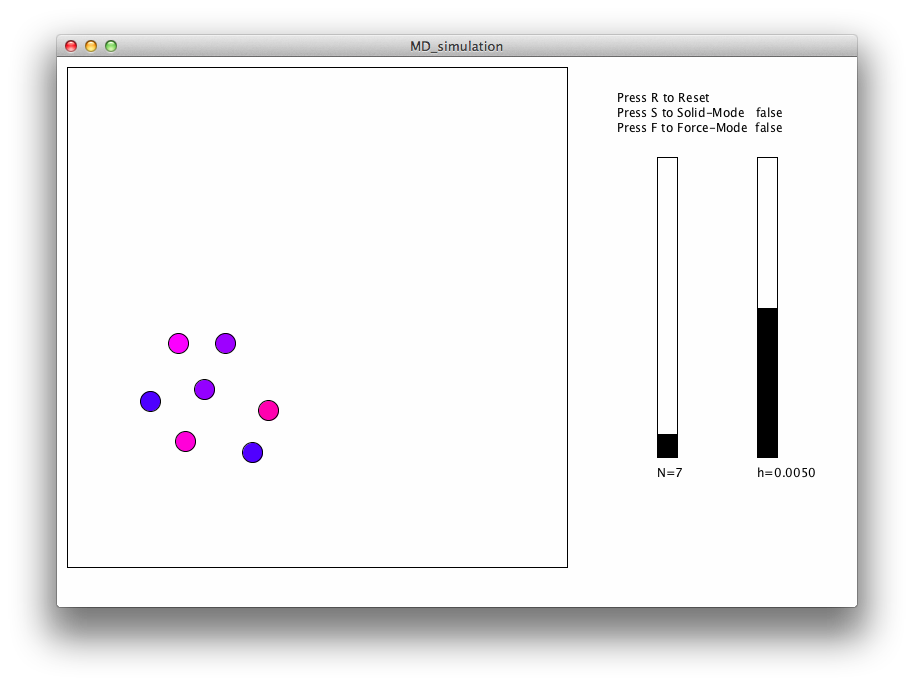
\includegraphics[width=150mm]{../result/cluster_picture.png}
 \end{center}
 \caption{クラスタの移動.}
 \label{fig:cluster}
\end{figure}


\newpage

図\ref{fig:solid}は凝固状態にしてしばらく実行し続けた結果であり,粒子が下の方に集まっていることが確認できる.これは粒子に下向きの力を継続的に加えて擬似的に凝固の現象を表現している.
これにより,粒子が自由に動き回る液体や気体の状態から,個体に移り変わる凝固現象の様子を確認できる.


\begin{figure}[htbp]
 \begin{center}
  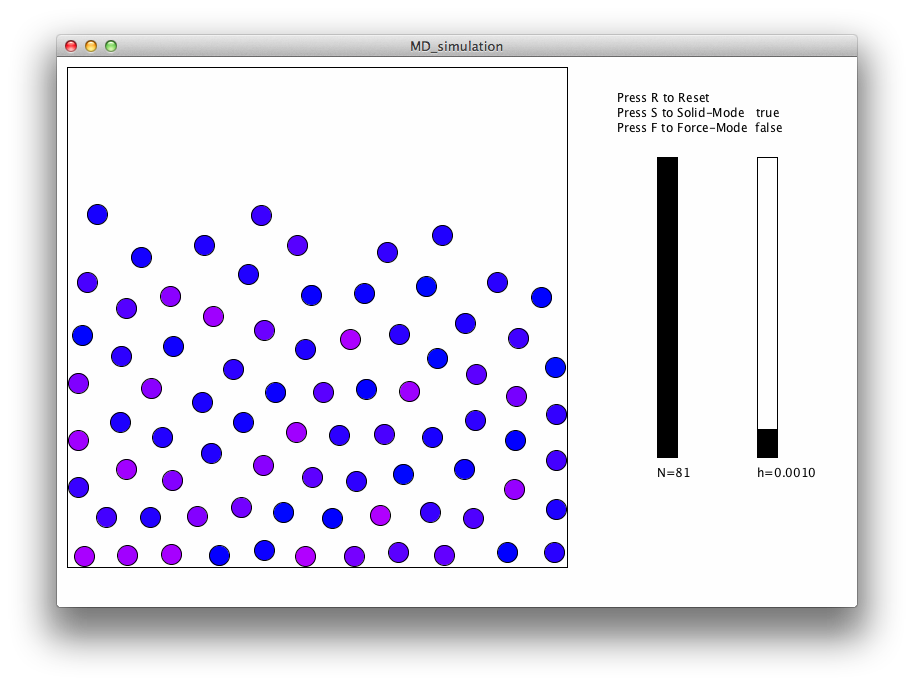
\includegraphics[width=150mm]{../implement/solid_mode.png}
 \end{center}
 \caption{凝固状態.}
 \label{fig:solid}
\end{figure}

\newpage

図\ref{fig:force}は粒子に加わる力を視覚化した状態であり,それぞれの粒子の中心から線が伸びている.
この線は長さが力の大きさ,向きが力の向きと対応しており力の加わり方をリアルタイムで把握することができる.
それぞれの粒子が力のパラメータを持っており,それらはシュミレーションの中で瞬時に変化していくため,値の確認は困難である.
しかし,この視覚化のおかげでそれぞれの粒子にかかる力を直感的に確認できる.

\begin{figure}[htbp]
 \begin{center}
  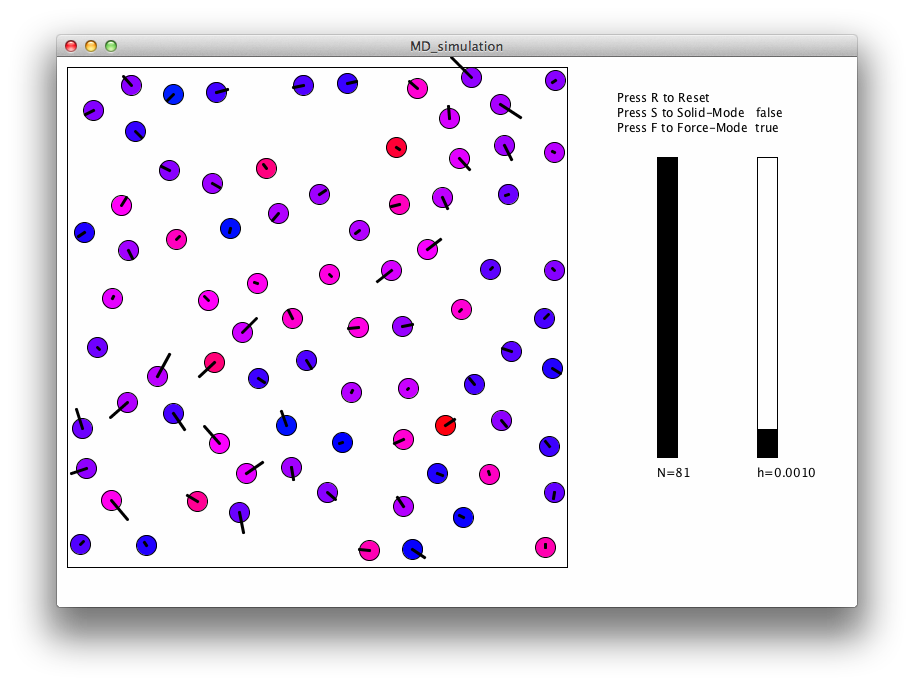
\includegraphics[width=150mm]{../implement/force_mode.png}
 \end{center}
 \caption{粒子に加わる力を視覚化した状態.}
 \label{fig:force}
\end{figure}


\end{comment}
%開発結果
\chapter{プログラムの制作過程と解説}
本章では,今回作成したプログラムのそれぞれの処理を解説する.(なぜ処理を解説するのかの理由はいるのか.なぜ処理を解説する章を書くのか?という理由)

\section{平面波の描写}
回折反射屈折の性質を可視化するためには多数の波を生成し,それらに重ね合わせの原理を適用しなければならない.そこで複数の点源から波を生成した上で,重ね合わせの原理によって生じた位相変化を視覚化するプログラムを作成した.

\subsection{波源から波の代わりとなる円を描写するプログラム}
最初はこれを実現するために,図\ref{fig:missdraw}のように,画面左上から右へ進行する斜めの線を入射波に見立て,入射波が波源として設定した座標を通過すると,波源から波の代わりとなる円を描写するプログラムを作成した.この後,円が重なった部分の色を変化させたり複数の円の包絡線を太く描写することを考えたが,計算が非常に複雑になること,処理速度が追いつかないことからこの方法は断念した.

\begin{figure}[htbp]
 \begin{center}
  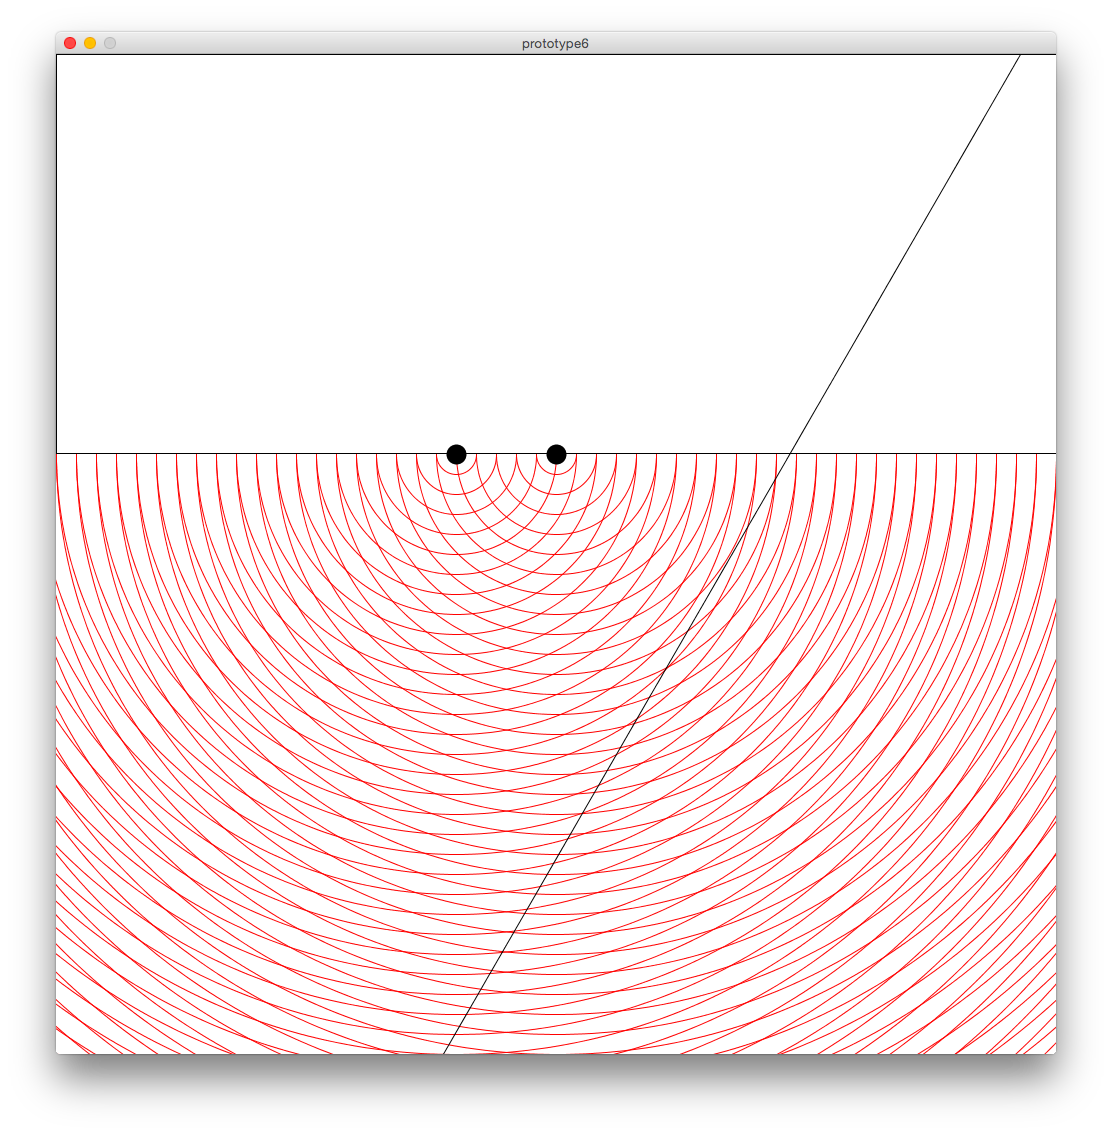
\includegraphics[width=70mm]{../implement/miss_draw.png}
 \end{center}
 \caption{波源から波に見立てた円を描写するプログラム.}
 \label{fig:missdraw}
\end{figure}

\newpage
そこで各ピクセルが波源からの距離,波源の生成された時間,波源から生成される波の波長と周期を基にして自らの地点の位相を計算する手法を考案した.

\subsection{平面波描写のアルゴリズム}
アルゴリズムは以下の手順である.
\begin{enumerate}
 \item 平面波の描写領域のピクセル数を指定しさらに位相計算を何ピクセルごとに行うかを指定する.この際指定したピクセル数をpoint\_regulationとする.
  \item 描写領域がクリックされると波源の座標情報が追加される.この際1つの波源ごとに,各ピクセルとの距離を計算し,配列に格納している.
  \item 点源とは異なる座標の点における変位の計算を全ての点源と全てのピクセルに対し行い,これによって得られた位相の値を各ピクセルごとに設けた配列に足し合わせていく.
  \item 各ピクセルごとの位相の値を基にして,値に応じた色の点を描写する.
 \item 3-4を繰り返して平面波の挙動を継続的に描写し続ける.
 \end{enumerate}

\subsection{画面のピクセル数を擬似的に変更する方法}

\subsection{点源とは異なる座標の点における変位の計算の実装}
物理学的背景の章で説明した(別の章の参照方法を調べる),点源とは異なる座標の点における変位の計算を行うためのElementary\_wavesクラスのメンバ関数,now\_displacement\_yは以下のように実装した.
\begin{screen}
{\small
\begin{verbatim}
  float now_displacement_y(float distance, float lambda, 
  float period, float time_adjustment){
    float time_phase_difference;
    time_phase_difference = 
    	((millis()-time_adjustment)/1000.0)*(360.0 / period);
    float a = (distance\%lambda)/lambda*(360.0);
    float y = sin(radians(-time_phase_difference+a));
    return y;
  }
\end{verbatim}}
\end{screen}

引数のdistanceにはある波源と,あるピクセルとの距離を代入する.
lambdaにはある波源から生成される波の波長,periodにはある波源から生成される波の周期を代入する.
time\_adjustmentにはある波源が生成された際に,プログラムを起動してから経過していた時間を代入する.

phase\_difference, a(変数名はのちのち変える)が物理学的背景の章で説明したどこに対応するのかを記す.

Processing言語にはプログラムが起動してからのミリ秒(1/1000秒)の数を返り値とするmillis()という関数が備えられている.(ここに引用元は必要なのか?processingのリファレンス)計算の都合上ミリ秒ではなく秒数に直した方が都合がいいので,5行目でmillisの値を1000で割っている.

7行目ではsin関数の中の値をradians()関数によって角度の単位を「度」からラジアンに変換している.Processingのパラメータの単位はラジアンなのでこのような処理を施している.











\begin{comment}





\begin{enumerate}
  \item 複数の粒子モデルを用意し,現在の座標、1つ前の座標,粒子に加わる力のパラメータを持たせる.
  \item Lennard-Jonesポテンシャルを用いて,粒子モデルに加わる力の合力を計算する.
  \item Verlet法を用いて次の座標を計算する.
  \item 2-3を繰り返して粒子モデルの座標を継続的に決定し続ける.
\end{enumerate}


\section{粒子の初期状態の設定}
粒子の座標,粒子にかかっている力を初期状態にする関数set\_particleは以下のように実装した.
\begin{screen}
{\small
\begin{verbatim}
void set_particle(){
  int i, j, k=0;
  for(i=1; i<10; i++){
    for(j=1; j<10; j++){
      if(k==n) break;
      ball_p[k][0] = i;
      ball_p[k][1] = j;
      pre_p[k][0] = i;
      pre_p[k][1] = j;
      k++;
    }
  }
  for(i=0; i<n; i++){
    ball_f[i][0] = 0; 
    ball_f[i][1] = 0;
  } 
} 
\end{verbatim}}
\end{screen}
変数i, jは粒子の座標を等間隔にするための任意の数値であり,kは粒子の番号,nは粒子の個数である.
粒子の数だけ,粒子の座標(ball\_p)と過去の座標(pre\_p)の初期値の格納を行い,粒子にかかっている力(ball\_f)を初期状態の0に設定している.
座標の初期値は左上から縦に9個ずつ等間隔に並ぶようになる.この関数はリセットにも用いられており,スライダーによって粒子の数が変更された際も実行される.

\section{粒子に加わる力}
ある一つの粒子に加わる力を決定するためには,他の粒子それぞれに対して力の計算を行い,それらの合力を求める必要がある.
\subsection{粒子間に加わる力の計算}
粒子間距離からLennard-Jonesポテンシャルを用いて,粒子に加わる力を求める.2粒子の座標からそれぞれの粒子に加わる力を計算する関数inter\_forceは以下ように実装した.
\begin{screen}
{\small
\begin{verbatim}
float[] lennard(float p1[], float p2[]){
  float d, force;
  float[] force_xy = new float[2];
  d = distance(p1, p2);
  force = -30 * pow(d,-13) + 30 * pow(d,-7);
  force_xy[0] = force * (p2[0] - p1[0])/d; 
  force_xy[1] = force * (p2[1] - p1[1])/d;
  return force_xy;  
}
\end{verbatim}}
\end{screen}
粒子の座標p1,p2を引数とし,p1に加わる力を返すようになっている.force\_xy[0]はx方向成分, force\_xy[1]はy方向成分である.
Lennard-Jonesポテンシャルによる力の計算は粒子間距離が1の時に力が0になるように定数を決めている.
粒子p2に加わる力はp1に加わる力の逆向きになるので以下のような実装を行う.
\begin{screen}
{\small
\begin{verbatim}
void inter_force(int i, int j){
  float[] tmp= new float[2];
  tmp = lennard(ball_p[i], ball_p[j]);
  ball_f[i][0] += tmp[0];
  ball_f[i][1] += tmp[1];
  ball_f[j][0] += -tmp[0];
  ball_f[j][1] += -tmp[1];
}
\end{verbatim}}
\end{screen}
2つの粒子の番号を引数とし,それらの粒子の座標を用いて関数lennardを実行し,結果をそれぞれのball\_fに格納している.後に複数の粒子との合力を求めるためにball\_fに対して加算代入(+=)を行う.
\subsection{合力の計算}
\begin{screen}
{\small
\begin{verbatim}
for( i=0; i<n-1; i++){
  for( j=i+1; j<n; j++){
    inter_force(i, j);
  }
}
\end{verbatim}}
\end{screen}
n個の粒子に対して重複を持たないように2粒子組み合わせを全て選択し,関数inter\_forceを実行している.これによりそれぞれの粒子のball\_fに,粒子間に加わる力が何度も加算代入され合力が求まる.

\section{粒子の動作}
粒子の座標の計算を行い,座標を更新することによって粒子を動かしていく.
\subsection{Verlet法による計算}
Verlet法を用いて粒子の座標を決定する.Verlet法の計算は以下のように実装した.
\begin{screen}
{\small
\begin{verbatim}
float[] verlet(float current[], float previous[], float force[]){
  float[] newpos = new float[2];
  newpos[0]=2*current[0]-previous[0]+h*h/m*force[0];
  newpos[1]=2*current[1]-previous[1]+h*h/m*force[1];
  return newpos;
} 
\end{verbatim}}
\end{screen}
Verlet法に従い,現在の座標(current),h時間前の座標(previous),粒子にかかっている力(force)を引数として,h時間後の座標(newpos)を返すようになっている.hは時間刻み,mは質量であり,それぞれグローバル変数で定義している.
\subsection{座標の更新}
Verlet法の計算結果から粒子の座標を更新する関数は以下のように実装した.
\begin{screen}
{\small
\begin{verbatim}
void calc_verlet(int i){
  float[] tmp= new float[2];
  if(solid_mode) ball_f[i][1]+= 0.00001/(h*h);//solid_mode
  tmp = ball_p[i];
  ball_p[i] = verlet(ball_p[i], pre_p[i],ball_f[i]);
  pre_p[i]= tmp; 
}
\end{verbatim}}
\end{screen}
i番目の粒子に対してVerlet法の計算を行い,計算結果から現在の座標(ball\_p)の更新を行う.Verlet法を繰り返し行えるように過去の座標(pre\_p)の更新も行う必要があり,tmpを用いて更新前のball\_pをpre\_pに格納している.

\section{粒子の描画}
粒子の座標が決定したので,粒子の描画を行う.また,粒子の速度によって色を変化させる.
\begin{screen}
{\small
\begin{verbatim}
void draw_particle(int i){
  float v;
  v = distance(ball_p[i], pre_p[i]);
  colorMode(HSB,360,100,100);
  fill(230+5000*v,100,100);  
  ellipse(ball_p[i][0]*50,ball_p[i][1]*50, ball_size*100,ball_size*100);
}
\end{verbatim}}
\end{screen}

\subsection{描画}
\begin{screen}
{\small
\begin{verbatim}
ellipse(ball_p[i][0]*50,ball_p[i][1]*50, ball_size*100,ball_size*100);
\end{verbatim}}
\end{screen}
粒子の描画はball\_p*50ピクセルの位置に円を描くというものになる.50倍するのはball\_pの値の範囲が0から10であり,粒子の動作範囲が500ピクセルの正方形であるからである.ball\_sizeは粒子のサイズを決定するグローバル変数である.

\subsection{粒子の色}
粒子の速度によって色を変化させる.色は速度が大きくなればなるほど,青から赤に変化するようにする.
\begin{screen}
{\small
\begin{verbatim}
  float v;
  v = distance(ball_p[i], pre_p[i]);
  colorMode(HSB,360,100,100);
  fill(230+5000*v,100,100); 
\end{verbatim}}
\end{screen}
粒子の現在の座標(ball\_p)と過去の座標(pre\_p)の距離を速度と考え,それに応じて色を変化させるようにしている.カラーモードをHSBに変更することによって,H(色相)の調整のみで青から赤に変化させる事が可能になる.

\begin{figure}[htbp]
 \begin{center}
  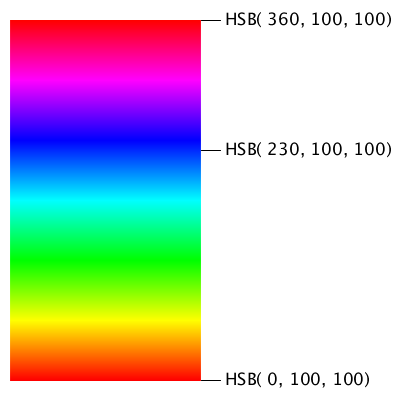
\includegraphics[width=80mm]{../implement/color_HSB.png}
 \end{center}
 \caption{HSBによる色の変化.}
 \label{fig:hsb}
\end{figure}
図\ref{fig:hsb}はS(彩度)=100,B(明度)=100の状態でH(色相)を変化させたときの色の変化を表している.粒子の色は230から360までの値をとり,青から赤に徐々に変化することが確認できる.

\section{壁との衝突}
粒子が動作範囲内の枠内を超えた場合,衝突判定を行い反射させる必要がある.判定を行う関数reflectは以下のように実装した.
\begin{screen}
{\small
\begin{verbatim}
void reflect(int i){
  if(ball_p[i][0]<ball_size){
  ball_p[i][0] = ball_size*2-ball_p[i][0];
  pre_p[i][0] = ball_size*2-pre_p[i][0];
  }  
  else if(ball_p[i][0]>10-ball_size){
    ball_p[i][0] = (10-ball_size)*2-ball_p[i][0];
    pre_p[i][0] = (10-ball_size)*2-pre_p[i][0];
  }

  if(ball_p[i][1]<ball_size){
    ball_p[i][1] = ball_size*2-ball_p[i][1];
    pre_p[i][1] = ball_size*2-pre_p[i][1];
  }
  else if(ball_p[i][1]>10-ball_size && solid_mode)
   ball_p[i][1]=10-ball_size-0.01;  
  else if(ball_p[i][1]>10-ball_size){
    ball_p[i][1] = (10-ball_size)*2-ball_p[i][1];
    pre_p[i][1] = (10-ball_size)*2-pre_p[i][1];
  }
}
\end{verbatim}}
\end{screen}
粒子iについて壁との衝突判定を行い,反射させている.衝突判定は上下左右の壁と行う必要があり,if文でそれぞれ行っている.
粒子の動きはVerlet法で定めているので,現在の座標(ball\_p)だけを更新しても,それ以降のVerlet法の計算に支障がでてしまう.そのため反射角が合うように過去の座標(pre\_p)の更新も行う.

\begin{figure}[htbp]
 \begin{center}
  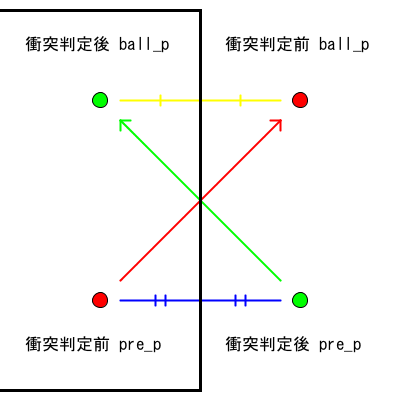
\includegraphics[width=80mm]{../implement/reflect_picture.png}
 \end{center}
 \caption{衝突判定時の座標の変換.}
 \label{fig:reflect}
\end{figure}

図\ref{fig:reflect}は衝突前後の粒子の座標を表しており,赤い粒子が衝突判定前,緑の粒子が衝突判定後を示しており,黄と青の線はそれぞれの粒子が壁と同じ距離であることを示している.
このような座標の変換をすることによって自然な衝突を表現できる.

\clearpage
\section{選択した粒子に力を加える}
クリックされた粒子にドラッグした方向の力を加えるようにし,ドラッグの距離によって力の大きさを変えるようにする.以下のように実装した.
\begin{screen}
{\small
\begin{verbatim}
int click_ball=0;

void mousePressed() {
  int i;
  for(i=0; i<n; i++){
    if(mouseX-10-20<=ball_p[i][0]*50 & mouseX-10+20>= ball_p[i][0]*50 &
    mouseY-10-20<=ball_p[i][1]*50 & mouseY-10+20>= ball_p[i][1]*50){
      click_ball = i;
      fill(0);
      //Ver Processing
      ellipse(pre_p[i][0]*50,pre_p[i][1]*50,ball_size*100,ball_size*100); 
      /*Ver JavaScript
      ellipse(10+pre_p[i][0]*50,10+pre_p[i][1]*50, 
       ball_size*100,ball_size*100);
       */
      mouse_p[0] = mouseX;
      mouse_p[1] = mouseY;
      return;
    }
  }
  click_ball = -1;
}
void mouseReleased(){
  if(click_ball != -1){
    ball_f[click_ball][0] +=( mouseX - mouse_p[0])*0.0001/(h*h);
    ball_f[click_ball][1] += (mouseY - mouse_p[1])*0.0001/(h*h);
  }
}
\end{verbatim}}
\end{screen}

\subsection{粒子の選択}
粒子がクリックされているかの判定を行い,クリックされていた場合,何番目の粒子か確認する必要がある.
また,選択された粒子がわかりやすいように黒く描画する.
\begin{screen}
{\small
\begin{verbatim}
void mousePressed() {
  int i;
  for(i=0; i<n; i++){
    if(mouseX-10-20<=ball_p[i][0]*50 & mouseX-10+20>= ball_p[i][0]*50 &
    mouseY-10-20<=ball_p[i][1]*50 & mouseY-10+20>= ball_p[i][1]*50){
      click_ball = i;
      fill(0);
      //Ver Processing
      ellipse(pre_p[i][0]*50,pre_p[i][1]*50,ball_size*100,ball_size*100); 
      /*Ver JavaScript
      ellipse(10+pre_p[i][0]*50,10+pre_p[i][1]*50, 
       ball_size*100,ball_size*100);
       */
      mouse_p[0] = mouseX;
      mouse_p[1] = mouseY;
      return;
    }
  }
  click_ball = -1;
}
\end{verbatim}}
\end{screen}
マウスボタンが押下された際に,i番目の粒子の上にマウスポインタが重なっているかの判定を行う.これをn個の粒子全てに対して行っていき
\begin{itemize}
  \item 重なりを確認した場合
\end{itemize}

\begin{enumerate}
 \setlength{\leftskip}{1.0cm}
  \item click\_ballに粒子の番号を格納する.
  \item その粒子を黒く描画する.
  \item マウスポインタの座標をmouse\_pに格納する.
  \item 関数mouse\_Pressedを終了する.
\end{enumerate}

\begin{itemize}
  \item 粒子全てに対して重なりを確認できなかった場合
\end{itemize}

\begin{itemize}
   \setlength{\leftskip}{1.0cm}
  \item click\_ballに-1を格納する.
\end{itemize}
この処理によりclick\_ballには選択された粒子の番号か-1が格納されている.また粒子が選択された場合,mouse\_pにはマウスポインタの座標が格納されている.これらの値はマウスが離された際の処理で利用する事になる.またProcessingとJavaScriptでの動作に異なりが生じるため変換を行う際は,プログラム内のコメントアウト部分の書き換えを行う必要がある.

\subsection{ドラッグ後の処理}
\begin{screen}
{\small
\begin{verbatim}
void mouseReleased(){
  if(click_ball != -1){
    ball_f[click_ball][0] +=( mouseX - mouse_p[0])*0.0001/(h*h);
    ball_f[click_ball][1] += (mouseY - mouse_p[1])*0.0001/(h*h);
  }
}
\end{verbatim}}
\end{screen}
マウスボタンが押された際に格納しておいたclick\_ball,mouse\_pを利用する.
マウスボタンが離された際にclick\_ballが-1以外(粒子が選択されている状態)であれば,ドラッグされた距離に応じてball\_f[click\_ball]に力を加える.このような実装を行う事でマウスボタンを用いて粒子を扱うことが可能になる.
また,格納する力の値を$h^2$で割っているのは時間刻みhの大きさに合わせて力の大きさを調整する必要があるからである.

\section{キー入力}
\begin{screen}
{\small
\begin{verbatim}
boolean solid_mode = false;
boolean force_mode = false;

void keyPressed() {  
  if (key == 's'||key == 'S') {
    if(solid_mode) solid_mode = false;
    else solid_mode = true;
  }
      if (key == 'f'||key == 'F') {
    if(force_mode) force_mode = false;
    else force_mode = true;
  }
  if (key == 'r'||key == 'R') set_particle();
}
\end{verbatim}}
\end{screen}
boolean変数がキー入力に対してtrue,falseと切り替わり,モード変更が可能になる.今回はSキーで凝固状態(solid\_mode),Fキーで力を視覚化した状態(force\_mode)の切り替えを行う.
またRキーはリセットに対応していて,粒子の状態を初期化する関数set\_particleを実行する.

\section{凝固状態}
凝固の現象を擬似的に表すために粒子に常に下向きの力を加え下層部に溜まるようにする.また,枠の下面部に粒子が衝突した際の反発力を減らす処理を行う.
\begin{itembox}[c]{関数calc\_verlet内 下向きの力を加える処理}
{\small
\begin{verbatim}
if(solid_mode) ball_f[i][1]+= 0.00001/(h*h);
\end{verbatim}}
\end{itembox}

\begin{itembox}[c]{関数reflect内 下面部の枠の反発力を減らす処理}
{\small
\begin{verbatim}
else if(ball_p[i][1]>10-ball_size && solid_mode)
 ball_p[i][1]=10-ball_size-0.01;
\end{verbatim}}
\end{itembox}
これらの処理はsolid\_modeがtrueの場合実行される.下面部の反発力を減らす処理では,粒子が下面部を通り越した際に,粒子のy座標に下面部と接触するようなy座標を格納している.これにより衝突後の反発力を減らすことができる.
この処理は粒子が壁と接触するように座標を決定するため反発力を0にしているように思えるが,継続的に下向きの力が加えられた状態でverlet法での計算が行われるため粒子に多少の上向きの動きが生じるようになる.
また,これを以下のように書き換えると反発力を0にすることができる.
\begin{screen}
{\small
\begin{verbatim}
else if(ball_p[i][1]>10-ball_size && solid_mode) {
  ball_p[i][1]=10-ball_size-0.01; 
  pre_p[i][1]=10-ball_size-0.01;   
}
\end{verbatim}}
\end{screen}
反発力を0にしてしまうと粒子が最下層に詰まってしまい粒子間距離が近すぎてしまう.この振る舞いは凝固の表現には不適切である.そのため,反発力を0にせずに少し減らす処理を選択した.

\section{力を視覚化した状態}
粒子に加わる力を線を用いて表す関数draw\_forceは以下のように実装した.
\begin{screen}
{\small
\begin{verbatim}
void draw_force(int i){
  float force_sqrt_x, force_sqrt_y;
  strokeWeight(3);
  if(ball_f[i][0]>0) force_sqrt_x = sqrt(abs(ball_f[i][0]));
  else force_sqrt_x = -sqrt(abs(ball_f[i][0]));
  if(ball_f[i][1]>0) force_sqrt_y = sqrt(abs(ball_f[i][1]));
  else force_sqrt_y = -sqrt(abs(ball_f[i][1]));
  line(ball_p[i][0]*50, ball_p[i][1]*50,
   ball_p[i][0]*50+force_sqrt_x, ball_p[i][1]*50+force_sqrt_y);
  strokeWeight(1);
}
\end{verbatim}}
\end{screen}
粒子iの座標(ball\_p[i][0]*50, ball\_p[i][1]*50)を始点とし,始点+粒子に加わっている力の根号(ball\_p[i][0]*50+force\_sqrt\_x ,ball\_p[i][1]*50+force\_sqrt\_y)まで太めの線(strokeWeight(3))の描画を行う.
粒子に加わっている力は振れ幅が大きいため根号を用いている.これにより1以下の小さな値の変化が確認しやすくなる.
粒子に加わる力には負の値も存在するが,根号の計算では負の値を扱うことができない.そのため,粒子に加わる力の絶対値から根号を求め,その値の符号を元の値と同一にする必要がある.
sqrt(abs(ball\_f[i][0]))はx方向に加わる力の絶対値の根号であり,粒子に加わる力の符号と同じになるようにforce\_sqrt\_xに格納している.
今回は線の長さに根号を用いているが,値をそのまま利用する方法もある.この方法には力の大きさが長さに比例するという利点があり,以下のように書き換えればよい.
\begin{screen}
{\small
\begin{verbatim}
line(ball_p[i][0]*50,ball_p[i][1]*50,
 ball_p[i][0]*50+ball_f[i][0],ball_p[i][1]*50+ball_f[i][1]);
\end{verbatim}}
\end{screen}



\section{スライダー}\label{sec:slider}
\begin{screen}
{\small
\begin{verbatim}
float slider_value = 1;
boolean slider_dragged = false;

void slider(int position_x, int position_y, int slider_height,
  int slider_width, int min, int max, int NumberOfTickMarks){
  
  int num_separator =
    (int)map(slider_value, min, max, 0, NumberOfTickMarks-1);
  float cordinate_y = position_y + slider_height - 
    ((float)slider_height / (NumberOfTickMarks-1))*num_separator;
  fill(255);
  rect(position_x, position_y, slider_width, slider_height);
  fill(0);
  rect(position_x, cordinate_y, slider_width, position_y +
    slider_height - cordinate_y);
  
  text( slider_value, position_x, position_y + slider_height + 20);
  
  
  if(mouseX >= position_x & mouseX <= position_x + slider_width &
    mouseY<=cordinate_y+10 & mouseY>= cordinate_y-10){
    if (mousePressed){
      slider_dragged= true;
    }
   }
  if(mousePressed==false) slider_dragged=false; 
   
   if(slider_dragged){
     num_separator+= (int)((cordinate_y - mouseY)/
       ((float)slider_height / (NumberOfTickMarks-1)));
     num_separator = constrain(num_separator, 0, NumberOfTickMarks-1);
     slider_value=map(num_separator, 0, NumberOfTickMarks-1, min, max);
   }
}
\end{verbatim}}
\end{screen}

\newpage

このプログラムを利用するためにはスライダーの値を格納する変数slider\_valueとスライダーのクリック判定を行う変数slider\_draggedをグローバル変数で定義する必要がある.
関数sliderの引数はスライダーの左上の座標を決定するposition\_x,position\_y,縦と横の幅を決定するslider\_height, slider\_width, 
値の最小値,最大値を決定するmin, max, 区切りの数を決定するNumberOfTickMarksとなり,それらを宣言することでスライダーを利用できる.
変数num\_separatorにはスライダーの一番下を0番目として区切りが下から何番目なのかを格納している.
この整数の値を利用することによってマウスをドラッグした際のスライダーの区切りを表現することができる.
以下にプログラムの処理の流れを記す.

\begin{enumerate}
  \item スライダーの値(slider\_value)から,区切りが下から何番目か(num\_separator)を計算する.
  \item 区切りの番号から,スライダー部分のy座標(cordinate\_y)を計算する.
  \item スライダーを描画する.
  \item スライダーの掴み判定(slider\_dragged)を行う.
   \item 掴み判定がtrueの場合
\end{enumerate}

\begin{enumerate}
   \setlength{\leftskip}{1.0cm}
  \item マウスの移動距離に合わせて区切りの番号に値を加える.
  \item 区切りの番号からスライダーの値を計算し格納する.
\end{enumerate}


\if0

\subsection{粒子の初期状態の設定}
\subsubsection{粒子の初期状態の設定}
\begin{screen}
{\small
\begin{verbatim}

\end{verbatim}}
\end{screen}
\fi



\end{comment}

%ソフトの振る舞い,ソフト試行錯誤の過程
\chapter{総括}
本研究では,複数の波源から生成される波が重ね合わせの原理により干渉する様子,回折現象,反射の法則,屈折の法則の視覚化プログラムの作成に取り組み,前者2つを完成させた.
それにより得られた成果を以下に示す.
\begin{enumerate}
  \item 任意の座標,時間に波源を生成し,生じる円形波の干渉の様子を確認できることや,波源ごとに波長,周期を調整できることから,波の挙動を直感的に理解しやすくなった.
  \item 数式等では特に説明し辛い,回折現象を視覚化することができた.
  \item プログラムのJavaScript化を行うことでタブレット上での動作が可能となり,今後教育現場で利用できる可能性を持たせた.
\end{enumerate}

今後の課題を以下に示す.
\begin{enumerate}
\item 反射角,屈折角を正確に表示できるようにするため,本研究のプログラムとは異なる反射波,屈折波の描写方法を考案しなければならない.
\item 教材として利用するには,スライダーの形等,デザイン性に欠ける部分がありこれらの改善を行わなければならない.
\end{enumerate}



%総括
\chapter*{謝辞} 
本研究を行うにあたり,終始多大なるご指導,御鞭撻をいただいた西谷滋人教授に対し,深く御礼申し上げます.また,本研究の進行に伴い,
様々な助力,知識の供給を頂きました西谷研究室の同輩,先輩方に心から感謝の意を示します.本当にありがとうございました.%謝辞


%参考文献

\begin{thebibliography}{9}
\bibitem{simizu}「ICT活用授業による学力向上に関する総合的分析評価」,清水康敬, 日本教育工学会論文誌 32(3), (2008), 293-303.
\bibitem{monbu}「教育の情報化ビジョン 〜21世紀にふさわしい学びと学校の創造を目指して〜」,文部科学省,\url{http://www.mext.go.jp/b_menu/houdou/23/04/__icsFiles/afieldfile/2011/04/28/1305484_01_1.pdf}, p34.
\end{thebibliography}

\end{document}




%終了